% Choose the language of your thesis passing 'french' or 'english' as
% \documentclass option.
% Note1: The 'page de garde' will always be written in French.
% Note2: You will have an error if you change the language of the document and
%        compile it without cleaning the auxiliary files. Compiling it again
%        should solve the problem.
\documentclass[english,a4paper,11pt,twoside,table]{StyleThese}
\newcommand{\included}{}

\usepackage{amsmath,amssymb}             % AMS Math
\usepackage[T1]{fontenc}
\usepackage[utf8x]{inputenc}
\usepackage{babel}
\usepackage{datetime}

\usepackage{lmodern}
\usepackage{tabularx}
%\usepackage{tabular}
\usepackage{multirow}

\usepackage{hhline}
\usepackage[left=1.5in,right=1.3in,top=1.1in,bottom=1.1in,includefoot,includehead,headheight=13.6pt]{geometry}
\renewcommand{\baselinestretch}{1.05}

% Table of contents for each chapter

\usepackage[nottoc, notlof, notlot]{tocbibind}
\usepackage{minitoc}
\setcounter{minitocdepth}{2}
\mtcindent=15pt
% Use \minitoc where to put a table of contents

\usepackage{aecompl}

% Glossary / list of abbreviations

\usepackage[intoc]{nomencl}
\iftoggle{ThesisInEnglish}{%
\renewcommand{\nomname}{Glossary}
}{ %
\renewcommand{\nomname}{Liste des Abréviations}
}

\makenomenclature

% My pdf code

\usepackage{ifpdf}

\ifpdf
  \usepackage[pdftex]{graphicx}
  \DeclareGraphicsExtensions{.jpg}
  \usepackage[a4paper,pagebackref,hyperindex=true]{hyperref}
  \usepackage{tikz}
  \usetikzlibrary{arrows,shapes,calc}
\else
  \usepackage{graphicx}
  \DeclareGraphicsExtensions{.ps,.eps}
  \usepackage[a4paper,dvipdfm,pagebackref,hyperindex=true]{hyperref}
\fi

\graphicspath{{.}{images/}}

%% nicer backref links. NOTE: The flag ThesisInEnglish is used to define the
% language in the back references. Read more about it in These.tex

\iftoggle{ThesisInEnglish}{%
\renewcommand*{\backref}[1]{}
\renewcommand*{\backrefalt}[4]{%
\ifcase #1 %
(Not cited.)%
\or
(Cited in page~#2.)%
\else
(Cited in pages~#2.)%
\fi}
\renewcommand*{\backrefsep}{, }
\renewcommand*{\backreftwosep}{ and~}
\renewcommand*{\backreflastsep}{ and~}
}{%
\renewcommand*{\backref}[1]{}
\renewcommand*{\backrefalt}[4]{%
\ifcase #1 %
(Non cité.)%
\or
(Cité en page~#2.)%
\else
(Cité en pages~#2.)%
\fi}
\renewcommand*{\backrefsep}{, }
\renewcommand*{\backreftwosep}{ et~}
\renewcommand*{\backreflastsep}{ et~}
}

% Links in pdf
\usepackage{color}
\definecolor{linkcol}{rgb}{0,0,0.4} 
\definecolor{citecol}{rgb}{0.5,0,0} 
\definecolor{linkcol}{rgb}{0,0,0} 
\definecolor{citecol}{rgb}{0,0,0}
% Change this to change the informations included in the pdf file

\hypersetup
{
bookmarksopen=true,
pdftitle="Évaluation de la sécurité des équipements grand public connectés à Internet",
pdfauthor="Yann BACHY", %auteur du document
pdfsubject="Thèse", %sujet du document
%pdftoolbar=false, %barre d'outils non visible
pdfmenubar=true, %barre de menu visible
pdfhighlight=/O, %effet d'un clic sur un lien hypertexte
colorlinks=true, %couleurs sur les liens hypertextes
pdfpagemode=None, %aucun mode de page
pdfpagelayout=SinglePage, %ouverture en simple page
pdffitwindow=true, %pages ouvertes entierement dans toute la fenetre
linkcolor=linkcol, %couleur des liens hypertextes internes
citecolor=citecol, %couleur des liens pour les citations
urlcolor=linkcol %couleur des liens pour les url
}

% definitions.
% -------------------

\setcounter{secnumdepth}{3}
\setcounter{tocdepth}{2}

% Some useful commands and shortcut for maths:  partial derivative and stuff

\newcommand{\pd}[2]{\frac{\partial #1}{\partial #2}}
\def\abs{\operatorname{abs}}
\def\argmax{\operatornamewithlimits{arg\,max}}
\def\argmin{\operatornamewithlimits{arg\,min}}
\def\diag{\operatorname{Diag}}
\newcommand{\eqRef}[1]{(\ref{#1})}

\usepackage{rotating}                    % Sideways of figures & tables
%\usepackage{bibunits}
%\usepackage[sectionbib]{chapterbib}          % Cross-reference package (Natural BiB)
%\usepackage{natbib}                  % Put References at the end of each chapter
                                         % Do not put 'sectionbib' option here.
                                         % Sectionbib option in 'natbib' will do.
\usepackage{fancyhdr}                    % Fancy Header and Footer

% \usepackage{txfonts}                     % Public Times New Roman text & math font
  
%%% Fancy Header %%%%%%%%%%%%%%%%%%%%%%%%%%%%%%%%%%%%%%%%%%%%%%%%%%%%%%%%%%%%%%%%%%
% Fancy Header Style Options

\pagestyle{fancy}                       % Sets fancy header and footer
\fancyfoot{}                            % Delete current footer settings

%\renewcommand{\chaptermark}[1]{         % Lower Case Chapter marker style
%  \markboth{\chaptername\ \thechapter.\ #1}}{}} %

%\renewcommand{\sectionmark}[1]{         % Lower case Section marker style
%  \markright{\thesection.\ #1}}         %

\fancyhead[LE,RO]{\bfseries\thepage}    % Page number (boldface) in left on even
% pages and right on odd pages
\fancyhead[RE]{\bfseries\nouppercase{\leftmark}}      % Chapter in the right on even pages
\fancyhead[LO]{\bfseries\nouppercase{\rightmark}}     % Section in the left on odd pages

\let\headruleORIG\headrule
\renewcommand{\headrule}{\color{black} \headruleORIG}
\renewcommand{\headrulewidth}{1.0pt}
\usepackage{colortbl}
\arrayrulecolor{black}

\fancypagestyle{plain}{
  \fancyhead{}
  \fancyfoot{}
  \renewcommand{\headrulewidth}{0pt}
}

%\usepackage{MyAlgorithm}
%\usepackage[noend]{MyAlgorithmic}
\usepackage[ED=MITT - STICRT, Ets=INSA]{tlsflyleaf}
%%% Clear Header %%%%%%%%%%%%%%%%%%%%%%%%%%%%%%%%%%%%%%%%%%%%%%%%%%%%%%%%%%%%%%%%%%
% Clear Header Style on the Last Empty Odd pages
\makeatletter

\def\cleardoublepage{\clearpage\if@twoside \ifodd\c@page\else%
  \hbox{}%
  \thispagestyle{empty}%              % Empty header styles
  \newpage%
  \if@twocolumn\hbox{}\newpage\fi\fi\fi}

\makeatother
 
%%%%%%%%%%%%%%%%%%%%%%%%%%%%%%%%%%%%%%%%%%%%%%%%%%%%%%%%%%%%%%%%%%%%%%%%%%%%%%% 
% Prints your review date and 'Draft Version' (From Josullvn, CS, CMU)
\newcommand{\reviewtimetoday}[2]{\special{!userdict begin
    /bop-hook{gsave 20 710 translate 45 rotate 0.8 setgray
      /Times-Roman findfont 12 scalefont setfont 0 0   moveto (#1) show
      0 -12 moveto (#2) show grestore}def end}}
% You can turn on or off this option.
% \reviewtimetoday{\today}{Draft Version}
%%%%%%%%%%%%%%%%%%%%%%%%%%%%%%%%%%%%%%%%%%%%%%%%%%%%%%%%%%%%%%%%%%%%%%%%%%%%%%% 

\newenvironment{maxime}[1]
{
\vspace*{0cm}
\hfill
\begin{minipage}{0.5\textwidth}%
%\rule[0.5ex]{\textwidth}{0.1mm}\\%
\hrulefill $\:$ {\bf #1}\\
%\vspace*{-0.25cm}
\it 
}%
{%

\hrulefill
\vspace*{0.5cm}%
\end{minipage}
}

\let\minitocORIG\minitoc
\renewcommand{\minitoc}{\minitocORIG \vspace{1.5em}}

\usepackage{multirow}
%\usepackage{slashbox}

\newenvironment{bulletList}%
{ \begin{list}%
	{$\bullet$}%
	{\setlength{\labelwidth}{25pt}%
	 \setlength{\leftmargin}{30pt}%
	 \setlength{\itemsep}{\parsep}}}%
{ \end{list} }

\newtheorem{definition}{Définition}
\renewcommand{\epsilon}{\varepsilon}

% centered page environment

\newenvironment{vcenterpage}
{\newpage\vspace*{\fill}\thispagestyle{empty}\renewcommand{\headrulewidth}{0pt}}
{\vspace*{\fill}}

\usepackage{tablefootnote}

\usepackage{hyperref}
\hypersetup{
     colorlinks   = true,
     citecolor    = violet
}
\usepackage{graphicx} % for pdf, bitmapped graphics files
\usepackage{amsmath} % assumes amsmath package installed
\usepackage{amssymb}  % assumes amsmath package installed
\usepackage{bm} % for using bold lowercase greek letters
\usepackage{array}
\usepackage{colortbl}	% to color table background
%\usepackage[table]{xcolor}
\usepackage{subfigure}  
\usepackage{tikz}
\newcommand{\tikzcircle}[2][red,fill=red]{\tikz[baseline=-0.5ex]\draw[#1,radius=#2] (0,0) circle ;}%
\definecolor{turquoise}{rgb}{0.28 1 0.92}
\input{rc_inertial_params/math_commands.tex}
\usepackage{epstopdf}
\usepackage[colorinlistoftodos,prependcaption,textsize=tiny]{todonotes}
\newcommand\explainmore[1]{\textcolor{red}{#1}}
\newcommand\refrephrase[1]{\textcolor{yellow}{#1}}
\newcommand\donerephrasing[1]{\textcolor{green}{#1}}

%DIF PREAMBLE EXTENSION ADDED BY LATEXDIFF
%DIF UNDERLINE PREAMBLE %DIF PREAMBLE
\RequirePackage[normalem]{ulem} %DIF PREAMBLE
\RequirePackage{color}\definecolor{RED}{rgb}{1,0,0}\definecolor{BLUE}{rgb}{0,0,1} %DIF PREAMBLE
\providecommand{\DIFadd}[1]{{\protect\color{blue}\uwave{#1}}} %DIF PREAMBLE
\providecommand{\DIFdel}[1]{{\protect\color{red}\sout{#1}}}                      %DIF PREAMBLE
%DIF SAFE PREAMBLE %DIF PREAMBLE
\providecommand{\DIFaddbegin}{} %DIF PREAMBLE
\providecommand{\DIFaddend}{} %DIF PREAMBLE
\providecommand{\DIFdelbegin}{} %DIF PREAMBLE
\providecommand{\DIFdelend}{} %DIF PREAMBLE
%DIF FLOATSAFE PREAMBLE %DIF PREAMBLE
\providecommand{\DIFaddFL}[1]{\DIFadd{#1}} %DIF PREAMBLE
\providecommand{\DIFdelFL}[1]{\DIFdel{#1}} %DIF PREAMBLE
\providecommand{\DIFaddbeginFL}{} %DIF PREAMBLE
\providecommand{\DIFaddendFL}{} %DIF PREAMBLE
\providecommand{\DIFdelbeginFL}{} %DIF PREAMBLE
\providecommand{\DIFdelendFL}{} %DIF PREAMBLE
%DIF END PREAMBLE EXTENSION ADDED BY LATEXDIFF


\begin{document}


\sloppy
\begin{document}
    
\include{page_de_garde}

\makeflyleaf

% \cleardoublepage

\dominitoc

\pagenumbering{roman}

% \cleardoublepage

% Here you can see an example of how to create text conditioned by the language
% variable. The \iftoggle command:
%
%   \iftoggle{ThesisInEnglish}{%
%   <your-text-in-english>
%   }{%
%   <your-text-in-french>
%   }
%
% will compile only one of the two blocks, depending on the variable you set at
% the beginning of this document. Language selection is managed this way in the
% formatAndDefs.tex file. You too can create sections of your thesis that is
% language dependend this way, although you probably won't need it. Another use
% of \iftoggle can be found at the end of this file.
\iftoggle{ThesisInEnglish}{%
\section*{Acknowledgments}
}{%
\section*{Remerciements}
}
A faire en dernier :-) 

\begin{vcenterpage}
\iftoggle{ThesisInEnglish}{%
\section*{Abstract}
}{%
\section*{Resume}
}
 Amidst a lot of research in motion planning and control in concern with robotic applications, the mankind has never reached a point yet, where the robots are perfectly functional and autonomous in dynamic settings. Though it is controversial to discuss about the necessity of such robots, it is very important to address the issues that stop us from achieving such a level of autonomy. Industrial robots have evolved to be very reliable and highly productive with more than 1.5 million operation robots in a variety of industries. These robots work in static settings and they literally do what it is programmed for specific usecases, though the robots are flexible enough to be programmed for a variety of tasks. This research work makes an attempt to address these issues that separate both these settings in a profound way with special focus on uncertainties. Practical impossibilities of precise sensing abilities lead to a variety of uncertainties in scenarios where the robot is mobile or the environment is dynamic. This work focuses on developing smart strategies to improve the ability to handle uncertainties robustly in humanoid and industrial robots. First, we focus on a dynamical obstacle avoidance framework proposed for industrial robots equipped with skin sensors for reactivity. Path planning and motion control are usually formalized as separate problems in robotics, though both fundamentally address the same issue. High dimensional configuration spaces, changing environment and uncertainties do not allow to plan real-time motion ahead of time requiring a controller to execute the planned trajectory. The fundamental inability to unify both these problems has led to handle the planned trajectory amidst perturbations and unforeseen obstacles using various trajectory execution and deformation mechanisms. The proposed framework uses 'Stack of Tasks', a hierarchical controller using proximity information with a point cloud based reactive path planner to avoid obstacles. Experiments are performed in UR5 robot to check the validity of the framework both in simulation and real robot. 

 Second, we focus on a strategy to model uncertainties of the inertial parameters of a robot for a humanoid robot specific to balancing task scenarios. Model-based control has become more and more popular in the legged robots community in the last ten years. The key idea is to exploit a model of the system to compute precise motor commands that result in the desired motion. This allows to improve the quality of the motion tracking, while using lower feedback gains, leading so to higher compliance. However, the main flaw of this approach is typically its lack of robustness to modeling errors. In this paper we focus on the robustness of inverse-dynamics control to errors in the inertial parameters of the robot. We assume these parameters to be known, but only with a certain accuracy. We then propose a computationally-efficient optimization-based controller that ensures the balance of the robot despite these uncertainties. We used the proposed controller in simulation to perform different reaching tasks with the HRP-2 humanoid robot, in the presence of various modeling errors. Comparisons against a standard inverse-dynamics controller through hundreds of simulations show the superiority of the proposed controller in ensuring the robot balance.


\end{vcenterpage}

\tableofcontents

\printnomenclature
% Use \mtcfixnomenclature below if you have a glossary (added with
% \printnomenclature above) and you're see a shift in the mini-table of
% contents at the begining of each chapter (example: no mini-toc in chapter 1;
% mini-toc of chapter 1 appearing in chapter 2; and so on).
%
% You should not use \mtcfixnomenclature if you have no glossary (that means,
% if you don't use \printnomenclature or if your glossary is empty).
\mtcfixnomenclature

\mainmatter

\ifdefined\included
\else
\documentclass[a4paper,11pt,twoside]{StyleThese}
\usepackage{amsmath,amssymb}             % AMS Math
\usepackage[T1]{fontenc}
\usepackage[utf8x]{inputenc}
\usepackage{babel}
\usepackage{datetime}

\usepackage{lmodern}
\usepackage{tabularx}
%\usepackage{tabular}
\usepackage{multirow}

\usepackage{hhline}
\usepackage[left=1.5in,right=1.3in,top=1.1in,bottom=1.1in,includefoot,includehead,headheight=13.6pt]{geometry}
\renewcommand{\baselinestretch}{1.05}

% Table of contents for each chapter

\usepackage[nottoc, notlof, notlot]{tocbibind}
\usepackage{minitoc}
\setcounter{minitocdepth}{2}
\mtcindent=15pt
% Use \minitoc where to put a table of contents

\usepackage{aecompl}

% Glossary / list of abbreviations

\usepackage[intoc]{nomencl}
\iftoggle{ThesisInEnglish}{%
\renewcommand{\nomname}{Glossary}
}{ %
\renewcommand{\nomname}{Liste des Abréviations}
}

\makenomenclature

% My pdf code

\usepackage{ifpdf}

\ifpdf
  \usepackage[pdftex]{graphicx}
  \DeclareGraphicsExtensions{.jpg}
  \usepackage[a4paper,pagebackref,hyperindex=true]{hyperref}
  \usepackage{tikz}
  \usetikzlibrary{arrows,shapes,calc}
\else
  \usepackage{graphicx}
  \DeclareGraphicsExtensions{.ps,.eps}
  \usepackage[a4paper,dvipdfm,pagebackref,hyperindex=true]{hyperref}
\fi

\graphicspath{{.}{images/}}

%% nicer backref links. NOTE: The flag ThesisInEnglish is used to define the
% language in the back references. Read more about it in These.tex

\iftoggle{ThesisInEnglish}{%
\renewcommand*{\backref}[1]{}
\renewcommand*{\backrefalt}[4]{%
\ifcase #1 %
(Not cited.)%
\or
(Cited in page~#2.)%
\else
(Cited in pages~#2.)%
\fi}
\renewcommand*{\backrefsep}{, }
\renewcommand*{\backreftwosep}{ and~}
\renewcommand*{\backreflastsep}{ and~}
}{%
\renewcommand*{\backref}[1]{}
\renewcommand*{\backrefalt}[4]{%
\ifcase #1 %
(Non cité.)%
\or
(Cité en page~#2.)%
\else
(Cité en pages~#2.)%
\fi}
\renewcommand*{\backrefsep}{, }
\renewcommand*{\backreftwosep}{ et~}
\renewcommand*{\backreflastsep}{ et~}
}

% Links in pdf
\usepackage{color}
\definecolor{linkcol}{rgb}{0,0,0.4} 
\definecolor{citecol}{rgb}{0.5,0,0} 
\definecolor{linkcol}{rgb}{0,0,0} 
\definecolor{citecol}{rgb}{0,0,0}
% Change this to change the informations included in the pdf file

\hypersetup
{
bookmarksopen=true,
pdftitle="Évaluation de la sécurité des équipements grand public connectés à Internet",
pdfauthor="Yann BACHY", %auteur du document
pdfsubject="Thèse", %sujet du document
%pdftoolbar=false, %barre d'outils non visible
pdfmenubar=true, %barre de menu visible
pdfhighlight=/O, %effet d'un clic sur un lien hypertexte
colorlinks=true, %couleurs sur les liens hypertextes
pdfpagemode=None, %aucun mode de page
pdfpagelayout=SinglePage, %ouverture en simple page
pdffitwindow=true, %pages ouvertes entierement dans toute la fenetre
linkcolor=linkcol, %couleur des liens hypertextes internes
citecolor=citecol, %couleur des liens pour les citations
urlcolor=linkcol %couleur des liens pour les url
}

% definitions.
% -------------------

\setcounter{secnumdepth}{3}
\setcounter{tocdepth}{2}

% Some useful commands and shortcut for maths:  partial derivative and stuff

\newcommand{\pd}[2]{\frac{\partial #1}{\partial #2}}
\def\abs{\operatorname{abs}}
\def\argmax{\operatornamewithlimits{arg\,max}}
\def\argmin{\operatornamewithlimits{arg\,min}}
\def\diag{\operatorname{Diag}}
\newcommand{\eqRef}[1]{(\ref{#1})}

\usepackage{rotating}                    % Sideways of figures & tables
%\usepackage{bibunits}
%\usepackage[sectionbib]{chapterbib}          % Cross-reference package (Natural BiB)
%\usepackage{natbib}                  % Put References at the end of each chapter
                                         % Do not put 'sectionbib' option here.
                                         % Sectionbib option in 'natbib' will do.
\usepackage{fancyhdr}                    % Fancy Header and Footer

% \usepackage{txfonts}                     % Public Times New Roman text & math font
  
%%% Fancy Header %%%%%%%%%%%%%%%%%%%%%%%%%%%%%%%%%%%%%%%%%%%%%%%%%%%%%%%%%%%%%%%%%%
% Fancy Header Style Options

\pagestyle{fancy}                       % Sets fancy header and footer
\fancyfoot{}                            % Delete current footer settings

%\renewcommand{\chaptermark}[1]{         % Lower Case Chapter marker style
%  \markboth{\chaptername\ \thechapter.\ #1}}{}} %

%\renewcommand{\sectionmark}[1]{         % Lower case Section marker style
%  \markright{\thesection.\ #1}}         %

\fancyhead[LE,RO]{\bfseries\thepage}    % Page number (boldface) in left on even
% pages and right on odd pages
\fancyhead[RE]{\bfseries\nouppercase{\leftmark}}      % Chapter in the right on even pages
\fancyhead[LO]{\bfseries\nouppercase{\rightmark}}     % Section in the left on odd pages

\let\headruleORIG\headrule
\renewcommand{\headrule}{\color{black} \headruleORIG}
\renewcommand{\headrulewidth}{1.0pt}
\usepackage{colortbl}
\arrayrulecolor{black}

\fancypagestyle{plain}{
  \fancyhead{}
  \fancyfoot{}
  \renewcommand{\headrulewidth}{0pt}
}

%\usepackage{MyAlgorithm}
%\usepackage[noend]{MyAlgorithmic}
\usepackage[ED=MITT - STICRT, Ets=INSA]{tlsflyleaf}
%%% Clear Header %%%%%%%%%%%%%%%%%%%%%%%%%%%%%%%%%%%%%%%%%%%%%%%%%%%%%%%%%%%%%%%%%%
% Clear Header Style on the Last Empty Odd pages
\makeatletter

\def\cleardoublepage{\clearpage\if@twoside \ifodd\c@page\else%
  \hbox{}%
  \thispagestyle{empty}%              % Empty header styles
  \newpage%
  \if@twocolumn\hbox{}\newpage\fi\fi\fi}

\makeatother
 
%%%%%%%%%%%%%%%%%%%%%%%%%%%%%%%%%%%%%%%%%%%%%%%%%%%%%%%%%%%%%%%%%%%%%%%%%%%%%%% 
% Prints your review date and 'Draft Version' (From Josullvn, CS, CMU)
\newcommand{\reviewtimetoday}[2]{\special{!userdict begin
    /bop-hook{gsave 20 710 translate 45 rotate 0.8 setgray
      /Times-Roman findfont 12 scalefont setfont 0 0   moveto (#1) show
      0 -12 moveto (#2) show grestore}def end}}
% You can turn on or off this option.
% \reviewtimetoday{\today}{Draft Version}
%%%%%%%%%%%%%%%%%%%%%%%%%%%%%%%%%%%%%%%%%%%%%%%%%%%%%%%%%%%%%%%%%%%%%%%%%%%%%%% 

\newenvironment{maxime}[1]
{
\vspace*{0cm}
\hfill
\begin{minipage}{0.5\textwidth}%
%\rule[0.5ex]{\textwidth}{0.1mm}\\%
\hrulefill $\:$ {\bf #1}\\
%\vspace*{-0.25cm}
\it 
}%
{%

\hrulefill
\vspace*{0.5cm}%
\end{minipage}
}

\let\minitocORIG\minitoc
\renewcommand{\minitoc}{\minitocORIG \vspace{1.5em}}

\usepackage{multirow}
%\usepackage{slashbox}

\newenvironment{bulletList}%
{ \begin{list}%
	{$\bullet$}%
	{\setlength{\labelwidth}{25pt}%
	 \setlength{\leftmargin}{30pt}%
	 \setlength{\itemsep}{\parsep}}}%
{ \end{list} }

\newtheorem{definition}{Définition}
\renewcommand{\epsilon}{\varepsilon}

% centered page environment

\newenvironment{vcenterpage}
{\newpage\vspace*{\fill}\thispagestyle{empty}\renewcommand{\headrulewidth}{0pt}}
{\vspace*{\fill}}

\usepackage{tablefootnote}

\usepackage{hyperref}
\hypersetup{
     colorlinks   = true,
     citecolor    = violet
}
\usepackage{graphicx} % for pdf, bitmapped graphics files
\usepackage{amsmath} % assumes amsmath package installed
\usepackage{amssymb}  % assumes amsmath package installed
\usepackage{bm} % for using bold lowercase greek letters
\usepackage{array}
\usepackage{colortbl}	% to color table background
%\usepackage[table]{xcolor}
\usepackage{subfigure}  
\usepackage{tikz}
\newcommand{\tikzcircle}[2][red,fill=red]{\tikz[baseline=-0.5ex]\draw[#1,radius=#2] (0,0) circle ;}%
\definecolor{turquoise}{rgb}{0.28 1 0.92}
\input{rc_inertial_params/math_commands.tex}
\usepackage{epstopdf}
\usepackage[colorinlistoftodos,prependcaption,textsize=tiny]{todonotes}
\newcommand\explainmore[1]{\textcolor{red}{#1}}
\newcommand\refrephrase[1]{\textcolor{yellow}{#1}}
\newcommand\donerephrasing[1]{\textcolor{green}{#1}}

%DIF PREAMBLE EXTENSION ADDED BY LATEXDIFF
%DIF UNDERLINE PREAMBLE %DIF PREAMBLE
\RequirePackage[normalem]{ulem} %DIF PREAMBLE
\RequirePackage{color}\definecolor{RED}{rgb}{1,0,0}\definecolor{BLUE}{rgb}{0,0,1} %DIF PREAMBLE
\providecommand{\DIFadd}[1]{{\protect\color{blue}\uwave{#1}}} %DIF PREAMBLE
\providecommand{\DIFdel}[1]{{\protect\color{red}\sout{#1}}}                      %DIF PREAMBLE
%DIF SAFE PREAMBLE %DIF PREAMBLE
\providecommand{\DIFaddbegin}{} %DIF PREAMBLE
\providecommand{\DIFaddend}{} %DIF PREAMBLE
\providecommand{\DIFdelbegin}{} %DIF PREAMBLE
\providecommand{\DIFdelend}{} %DIF PREAMBLE
%DIF FLOATSAFE PREAMBLE %DIF PREAMBLE
\providecommand{\DIFaddFL}[1]{\DIFadd{#1}} %DIF PREAMBLE
\providecommand{\DIFdelFL}[1]{\DIFdel{#1}} %DIF PREAMBLE
\providecommand{\DIFaddbeginFL}{} %DIF PREAMBLE
\providecommand{\DIFaddendFL}{} %DIF PREAMBLE
\providecommand{\DIFdelbeginFL}{} %DIF PREAMBLE
\providecommand{\DIFdelendFL}{} %DIF PREAMBLE
%DIF END PREAMBLE EXTENSION ADDED BY LATEXDIFF


\begin{document}


\sloppy
\begin{document}
\fi
\chapter*{Introduction}
\addstarredchapter{Introduction} 
Autonomy is undoubtedly the main goal in Robotics. We would like to develop robots which are self-reliant with supporting technologies to be as generic as possible. Every incremental research in robotics  directly or indirectly strives to automatize certain processes or mechanisms that solve a problem of physical interaction efficiently and effectively. Though it is controversial to talk about the need of such autonomy in robots, it is an undeniable fact that the research tries to solve robotic problems using algorithms with genericness and self-reliance. Autonomy is not only about robot having higher awareness and control on itself in ideal or pre-designed environments but also the ability to cope up with new and dynamic environments with ease. Developing algorithms with an ability to change, adapt or be flexible is the core problem of establishing autonomy in robots. 

In this thesis, we address two specific problems which comes under this futuristic vision of establishing advanced autonomy in robot control:\textit{Variability} in environment and \textit{Uncertainty} in robot model. By the term \textit{Variability}, we refer to environments of being in state of inconsistency or lack of fixed pattern for which an appropriate algorithm should be flexible enough to adapt without compromising on the final goal. Whereas by the term \textit{Uncertainty}, we refer to the incomplete knowledge of qualitative or quantitative aspects of a robot requiring a control algorithm to succeed in goals even without complete knowledge. Though these two terms look like they are very related to each other and it might even mean the same in some scenarios, they are fundamentally different and need to be handled differently. Both these problems are addressed in two different robotic platforms motivated by the current need of the hour in robotics research and development.

The first part of the thesis presents the development of a controller framework in industrial robots to handle variability in environment. Industrial robots work in static settings and they literally do what it is programmed for specific use-cases, though the robots are flexible enough to be programmed for a variety of tasks. This work makes an attempt to address these issues that separate both these settings in a profound way with special focus on dynamic obstacle avoidance where the robots encounter unforeseen obstacles while executing a desired task. 
The second part of the thesis presents the development of a robust controller for humanoid robot to ensure balance even when there is no absolute knowledge of the robot model. Lack of precise sensing abilities lead to a variety of uncertainties in robot model and the environment. In legged robots, due to the tree-like kinematic chain and the dynamic complexity, it is necessary to approximate the robot to a simple model for balance control. Unfortunately, it is quite sensitive to uncertainties of the model for which a robust control strategy is proposed to improve balance control amidst inertial uncertainties of the robot.

This thesis in short focuses on developing smart strategies to improve the ability to handle variability and uncertainties robustly both in humanoid and industrial robots respectively. The contributions of this thesis are:
\begin{itemize}
    \item A strategy to model uncertainties of the inertial parameters of a robot for a humanoid robot specific to balancing task scenarios.
    \item A dynamic obstacle avoidance framework proposed for industrial robots equipped with skin sensors for reactivity. 
\end{itemize}

In this chapter, we introduce the field of both industrial \& humanoid robots and the issues we face to motivate the need to solve variability and uncertainties specific to the context of this thesis. 
\section{Industrial Robots}
\subsection{History of Industrial Robots}
The idea of automatic machines has been in existence since many centuries with documented illustrations of robots, automata in various interesting applications. Archytas (4th century B.C), the founder of mathematical mechanics, invented an autonomous wooden flying pigeon powered by steam. Fig.~\ref{fig:automatons0} (a) shows this mechanical bird which can fly uninterrupted for hundreds of meters and is considered to be the first ever robot documented. Another interesting application shown in Fig.~\ref{fig:automatons0} (b) is an analog computer (developed during 1st century B.C) that can predict astronomical positions for the purpose of maintaining a calendar and astrological reasons. It has 37 gears enabling the device to track the moon and sun positions keeping track of time. Hydro powered clocks was common in China since the 40th century B.C to study astronomical positions. Fig.~\ref{fig:automatons0} (c) shows Su Song's artistic clock tower developed in 10th century A.D with mechanically controlled mannequins chiming and ringing bells. Al Jazari in the muslim world is known for developing hydro powered automatic machines such as the drink-serving waitress, hand washing automaton, peacock fountain. Though it might look trivial, the works were known for its creative mechanisms, components and design features. Cam \& crank shafts, escapement mechanism in rotating wheels, segmental gears are some of his contributions which are still used in modern mechanical devices today \cite{hill2012book}.  

\begin{figure*}[!tbph]
\begin{subfigure}
[Archytas' bird]{\includegraphics[width=4.1cm,height=5.5cm]{chapters/intro/images/pigionsteam.jpg}}\quad
\end{subfigure}
\begin{subfigure}
[Antikythera mechanism]{\includegraphics[width=4.3cm,height=5.5cm]{chapters/intro/images/machineanti.jpg}}\quad
\end{subfigure}
\begin{subfigure}
[Su Song's Clock Tower]{\includegraphics[width=4.1cm,height=5.5cm]{chapters/intro/images/clocktower.JPG}}\quad
\end{subfigure}
\caption{Automatons in the ancient world}
\label{fig:automatons0}
\end{figure*}

Fig.~\ref{fig:automatons1} (a) shows the first ever humanoid robot in the records, designed by Leonardo da Vinci. This mechanical knight has joints similar to human beings with an ability to perform motions such as waving the arms, moving the head and jaws, sitting and standing up. Around 18th century many automatons were developed capable of entertaining, speaking and playing musical instruments. One such musical automaton in the form of an elephant shown in the Fig.~\ref{fig:automatons1} (b) is designed by Hubert Martinet, a french clockmaker in 1774. Another interesting automaton in the Fig.~\ref{fig:automatons1} (c) is the \textit{Digesting Duck} made by Jacques de Vaucanson. This golden mechanical duck imitates the ability to eat and defecate grains.

\begin{figure*}[!tbph]
\begin{subfigure}
[Da Vinci's robot]{\includegraphics[width=4cm,height=4.5cm]{chapters/intro/images/leorobot.jpg}}\quad
\end{subfigure}
\begin{subfigure}
[Elephant Automaton]{\includegraphics[width=4cm,height=4.5cm]{chapters/intro/images/elephantAutomaton.jpg}}\quad
\end{subfigure}
\begin{subfigure}
[Digesting Duck]{\includegraphics[width=4cm,height=4.5cm]{chapters/intro/images/duck.jpg}}\quad
\end{subfigure}
\caption{Automatons in the 18th Century}
\label{fig:automatons1}
\end{figure*}

% May be talk about Remote-controlled systems

Though most of the automatons were created for fun or artistic satisfaction in the beginning, the characterization of robots to be human look-alike machines that can serve human beings came up in the 20th century. The term \textit{robot} itself was born in 1921 from R.U.R (Rossum's Universal Robots), a czech play written by Karel Čapek. The play depicts robots as good and benevolent workers serving the human beings later gaining super human strength to revolt humans leading to end of life. This negative idea changed after a russian writer, Isaac Asimov made a contrasting characterization of robots as just mechanical creatures with no emotions. Asimov's laws of robotics in 1942 gave way to a new perspective of robots to be seen as an product that could be developed by engineers to improve productivity in manufacturing industries. During the same time period, a programmable mechanism to do spray painting was designed by Pollard and Roselund for DeVilbiss, the first industrial robot supplier. The mechanism is based on pantograph pivoted on two rotary actuators on a fixed base. 


\begin{figure*}[!tbph]
\centering
\begin{subfigure}
[Pollard's Paint Sprayer]{\includegraphics[width=6.5cm,height=6cm]{chapters/intro/images/pollard.png}}
\end{subfigure}
\begin{subfigure}
[Unimate Robot's Television Appearance]{\includegraphics[width=6.5cm,height=6cm]{chapters/intro/images/unimate.jpg}}
\end{subfigure}
\caption{Robotic Mechanisms in the Beginning}
\label{fig:robotmechanisms}
\end{figure*}


In 1954, George Devol developed the the first truly programmable robot UNIMATE which originally consisted of an arm and a drum memory box with pre-programmed tasks. A collaboration with Joseph Engelberger, the father of robotics gave birth to \textit{Unimation}, the first company to make robots which were used to transport and weld die castings on auto bodies preventing humans from dangerous working conditions. Though the numerically controlled turning \& milling machines and the hydraulic assembly machines were programmable, the industrial robots differed in the sophistication of reprogrammability and the versatility to be used for different tasks. This is purely because of the invention of digital computers and integrated circuit technology which allowed to develop the brains of industrial robots.

\begin{figure}[h]
\centering
{\includegraphics[scale=1]{chapters/intro/images/gm.jpg}}
\caption{Manufacturing unit in General Motors with 'Unimate' robots in 1969}
\label{fig:unimate}
\end{figure}

Ford director Del Harder's interest to install 2000 unimation robots triggered American manufacturing industries to pay attention to the robotics industry a bit more seriously. Installations in General Motors in Ohio, US in the beginning of 1960s marks the real beginning of industrial robotics. After an intense research and development during the next 15 years and the introduction of micro-processors provided the basis for low cost control systems. A norwegian company \textit{Trallfa} designed and developed a cost-effective alternative to Unimate robots for spray painting applications. Several companies such as \textit{Electrolux, ESAB, Atlas Copco,} and \textit{ASEA} followed the same path designing in house robots for their own purposes which suited the requirements of other customers resulting in a product of its own. This phenomenon gave birth to more than 70 robot manufacturers by the year 1973.



The industrial robots were hydraulic or pneumatic in the beginning though they are very suitable for heavier loads. Vicarm in 1968 turned out to be the first electric robot to suit the lighter loads of assembly lines and arc welding. The 6 degree of freedom robot (5 revolute + 1 prismatic) was designed with simplified analytic solutions by Victor Scheinman allowing the robot to track arbitrary paths in the work space of the robot. Cincinnati Milacron, the largest machine tool constructor during the 1970s developed the "The Tomorrow Tool", the first microcomputer based robot. The robots in the beginning were used for simple tasks such as pick and place with no external sensing. External sensing along with the ability of robots to perform advanced motion behaviors gave rise to complex applications like welding, grinding and deburring. The applications can be divided to three main categories: Assembly lines, process operations and material handling. The main motivation of industrial robotics is to apply productive, cost-effective and human safe automation solutions without compromising on the quality of the products. 


The capabilities of robots were purely driven by the manufacturing industries with different industries focusing on different requirements. Material handling required robots of increased loading capacity while arc welding and motion dependant applications required the robot to have better electrical motors and path control. In the beginning of 1980s the assembly lines were mostly focused and shorter cycle time has always been the goal which required robots to be highly dynamic and repeatable. Metal industries required the robots to be very stubborn to work in hot and unsafe working environments. Though robots had complex applications, simple applications such as picking and placing, material transportation were economical for automization. 
These customer demands provided way to the industrial robotic revolution in the 1980s. 


\begin{figure}[!tbph]
\begin{subfigure}
[The Tomorrow Tool-T3]{\includegraphics[width=4.3cm,height=6cm]{chapters/intro/images/t3.jpg}}\quad
\end{subfigure}
\begin{subfigure}
[Shakey]{\includegraphics[width=4.1cm,height=6cm]{chapters/intro/images/Shakey.jpg}}\quad
\end{subfigure}
\begin{subfigure}
[Stanford Arm]{\includegraphics[width=4.1cm,height=6cm]{chapters/intro/images/stanfordarm.JPG}}\quad
\end{subfigure}
\caption{Automatons in the ancient world}
\label{fig:robots}
\end{figure}

Robotics was unanimously accepted as a key focus area to increase industrial development and achieve competitive edge. Advanced sensors such as force sensors, vision cameras and laser scanners were introduced in the late 1980s
to make physical interactions with the environment to improve the intelligence. It is necessary to make deeper connections with the control system to make intelligent decisions in the working environment. Though the vision of robotics in the 1980s was very ambitious to automise factories completely with robots and less human labour, it was very soon realized that robotics being a multi-disciplinary technology is not so easy and certain human work mechanisms are difficult to be replicated. Heterogenous integration of complex systems involves a lot of problems and developing a robotic workcells are more expensive than the workers themselves though they are economically feasible for simpler tasks.

Productivity is a complex concept and the idea of robots solely responsible for improving productivity changed in the beginning of 1990s. The dependence on robotics for more ambitious tasks started to decrease though it was and still an inevitable part of the mechatronic technology to automize and improve productivity. Now robotics are used for medical applications, service, entertainment and disaster handling applications. Though the industrial robots have been in use for quite a long time, there are many challenges not addressed until now. This is where the 'Factory in a Day' project comes into picture.

\subsection{'Factory in a Day' project}
We are aware that robot automation has been into existence since the 1960s and has seen a lot of technological advancements but they are still challenged by installation time and cost involved in setting up robots specific to the functional needs in factories. There is a lot of risk involved in such investment making it economically less attractive to smaller companies. Moreover, the factory setups are fixed environments with hard coded settings of millimeter precision so that they are perfectly under control at all times. Floating robot bases introduces errors and uncertainties which requires more robust components to handle factory scenarios. There is also a big concern in safety of human beings working in robot environments. Though recent technologies are focused towards collaborative robot control where human beings and robots can work together, these algorithms are either completely not matured to be used in factories or not yet known in the industrial community. This thesis is funded by Factory-in-a-Day project which focuses on these issues mentioned above.

Factory-in-a-Day project puts forward the idea of minimizing the installation time and the cost involved from several months to just a single day. The project focuses on the following aspects of robotics which is synonymous to the steps taken in a day to install a robotic setup. 

\begin{itemize}
\item Standardized procedures to design 3D printed custom parts which are usually attached with an existing robot arm and grippers using novel templates to minimize the time taken.
\item The flexibility to be placed in factories without any alteration where intelligent self-calibration and an adaptive framework that helps to connect with the existing machineries in ease.
\item Use rapid teaching to program production tasks in the setup from a rich set of learnable skills
for applications like mould finishing, welding and assembly.
\item Visually intuitive tools for the workers in the factory to assess robot's behavior motion behaviors. Augmented reality can be used to visualize the robot's intended path by wearing a glass to be aware of its activity to be collaborative in nature.
\item A mature human-robot interaction framework to allow the humans collaborate with robots in an unfenced workspace using a dynamic obstacle avoidance framework with proximity skin sensors and 
reactive path planning and control algorithms.
\end{itemize}
The above aspects along with proposed certification procedures and a complete focus on manufacturing industry can radically change the automation sector. The work done in this thesis orients in the direction of the last aspect which is human-robot collaboration. The Fig.~\ref{fig:doa_motivation} (a) shows the reality of many robotics based manufacturing units with fences avoiding dangerous accidents with human beings. There are strict protocols followed to get inside the fence incase of repairs needed. It is definitely not productive, and the new age robot manufacturers such as \textit{Universal Robots} focus on manufacturing robots with safe touch control which allows the robot to stop when the human is in contact. In case the robots are moving fast, they can be programmed to adapt/reduce the speed by monitoring the presence of human beings using laser scanners. Though there are systematic hacks available, the thesis supports the idea of human-robot collaboration in the real sense where they share the workspace with more awareness about the environment and task scenarios. 
\begin{figure}[!tbph]
\begin{subfigure}
[Fenced Robot for Safety]{\includegraphics[width=6.6cm,height=6cm]{chapters/intro/images/fencedrobot.png}}\quad
\end{subfigure}
\begin{subfigure}
[New Gen Universal Robot]{\includegraphics[width=6.5cm,height=6cm]{chapters/intro/images/urcorobot.jpg}}\quad
\end{subfigure}
\caption{Motivation towards Collaborative Robots}
\label{fig:doa_motivation}
\end{figure}


\section{Humanoid Robots}
Humanoid Robots are robotic mechanisms resembling the kinematics of human beings with a head and a torso bridging two arms \& two legs. There are many variants modeling only certain parts of the human body though we stick with the context of legged robots with arms through out this report. Building humanoid robots require the need of understanding human behaviors and kinematic structure deeply. Attempting to build such robots sometimes give us better understanding of human beings making the knowledge flow between both the domains bi-directional. The anthropomorphic design of humanoids also help in getting the acceptance of people as a social entity making the human-robot interaction feasible \cite{fink2012anthropomorphism}. Also the physical ability of humanoids make them suitable for rescue or disaster handling scenarios. The social acceptance and the physical ability of humanoids make them a very good platform to invest on researching technologies that improve the intelligence of such robots.

\subsection{History of Humanoid Robots}
Humanoid robots were just controlled using traditional joint position control methodologies like in industrial robots though there is a need for stiff drive train for precision. WABOT-1 was the first humanoid robot to walk, communicate, visually recognize objects and manipulate them. The robot was built by Kato's lab from University of Waseda in 1973 \cite{kato1973development}. The same lab lead a series of developments achieving the latest one WABIAN-2 which can walk with stretched knees \cite{ogura2006development}. Chronologically WABOT-1 was followed by P2, the first robot to perform stable walking, was launched in 1996 by Honda after 10 years of modular and systematic research focused on dynamic biped walking and stability control \cite{hirai1998development}. The next version P3  was much lighter and gave way to the launch of the famous ASIMO robot in 2000 with a more friendly appearance and improved intelligence \cite{hirose2007honda}. ASIMO's impressive capabilities attracted the attention of robotics researchers and created a perspective of humanoid robots to be exploited for service robotics \cite{kaneko2009cybernetic}. 


\begin{figure}[!tbph]
\begin{subfigure}
[WABOT-1]{\includegraphics[width=4.1cm,height=6cm]{chapters/intro/images/wabot1.jpg}}\quad
\end{subfigure}
\begin{subfigure}
[ASIMO]{\includegraphics[width=4.2cm,height=6cm]{chapters/intro/images/asimo.jpg}}\quad
\end{subfigure}
\begin{subfigure}
[Kobian]{\includegraphics[width=4.2cm,height=6cm]{chapters/intro/images/kobian.jpg}}\quad
\end{subfigure}
\caption{Humanoids of the first generation}
\label{fig:hr_first}
\end{figure}


Japan took the trigger seriously and many humanoids were developed in the last decade both for entertainment and demonstrating physical capabilities. Different sized humanoids with great capabilities were built within the \textit{Humanoid Robotics Project} by Kawada Industries and Japanese National Institute of Advanced Industrial Science and Technology (AIST)  with the first prototype HRP-2P launched in 2002 \cite{kaneko2002design} followed by HRP-2 \cite{Kaneko04humanoidrobot}, HRP-3 \cite{kaneko2008humanoid} in the next years. HRP-4C in 2009 \cite{kaneko2009cybernetic}, assumes a feminine appearance while the latest HRP4 in 2010, is more athletic and light \cite{kaneko2011humanoid}. Sony launched QRIO (previously called SDR-3X), a small humanoid robot for entertainment in 2004 \cite{geppert2004qrio}. Fujitsu Automation also launched a series of small humanoid robots HOAP with the latest version HOAP-3 released in 2005. Other japanese robots include H7  from the University of Tokyo \cite{nishiwaki2007experimental}, Kenta, a musculo-skeletal robot \cite{inaba2003building}, Kojiro in 2007 \cite{mizuuchi2007advanced},Kenshiro in 2012 \cite{nakanishi2012design}. Schaft launched one of the most powerful humanoid robots inspired from HRP-2 series robots in 2013.

The Korea Advanced Institute of Science and Technology (KAIST) invested in developing several versions of KAIST humanoid robots(KHR) since 2002 with the latest one released in 2011 with the name HUBO 2 \cite{kim2002development,park2005mechanical,park2005development,grey2013multi}. The other well known network based robots from Korea are the MAHRU and AHRA series \cite{you2005network,kwon2007biped, kim2011providing}. Technical Unversity of Munich (TUM) built the humanoid robot Johnnie \cite{gienger1999design} followed by an improved version called Lola \cite{lohmeier2009humanoid} known for its fast and robust motions. The Italian Institute of Technology (IIT)  built a torque controlled iCub \cite{metta2010icub} and COMAN in 2012
\cite{tsagarakis2013compliant}. The University Carlos III from Spain, built the Rh-1 in 2007 \cite{arbulu2007real} and its successor TEO in 2011 \cite{monje2011full}. Pal Robotics also built the humanoid robots REEM-B \cite{tellez2008reem}, REEM-C, a human friendly design in 2014 \cite{robotics2014reem}. In 2007, Aldebaran Robotics, a french company launched Nao, one of the most popular small humanoid robot in the world motivated several laboratories to do research on humanoids with less investment \cite{gouaillier2009mechatronic}. The same company presented a torque controlled child-size robot Romeo. 

\begin{figure}[h]
\begin{subfigure}
[HRP2]{\includegraphics[width=4.4cm,height=6cm]{chapters/intro/images/hrp2.jpg}}\quad
\end{subfigure}
\begin{subfigure}
[Kojiro]{\includegraphics[width=4cm,height=6cm]{chapters/intro/images/kojiro.jpg}}\quad
\end{subfigure}
\begin{subfigure}
[Kenshiro]{\includegraphics[width=4.1cm,height=6cm]{chapters/intro/images/kenshiro.png}}\quad
\end{subfigure}
\caption{Japanese Humanoids }
\label{fig:hr_second}
\end{figure}

SARCOS Research Corporation and ATR (Advanced Telecommunications Research Institute International) from Japan built robots Erato DB (Dynamic Brain) based on hydraulic actuation in 2000 \cite{atkeson2000using}, and CBi in 2006 \cite{cheng2007cb} which explores the background neural processes in the human brain. DARPA Robotics Challenge (DRC), a competition funded by US Defense Advanced Research Projects Agency (DARPA)  was held between 2012-2015 motivated the development of humanoid robots in the US.  CHARLI in 2010 \cite{knabe2013team}, THOR in 2014 \cite{yi2015team}, CHIMP in 2013 \cite{stentz2015chimp}, Valkyrie in 2013 \cite{radford2015valkyrie} are some popular robots in the US.Most of the robots presented above are fully actuated electrical systems which usually compose rigid bodies with compliance only in the foot to handle contact impacts from the ground while walking. Also they mostly use the traditional high-gain position control methodologies which requires a precise robot dynamic model and Zero Moment Point (ZMP) concept by Vukobratovic \cite{vukobratovic1972stability} is applied in the control of many bipeds \cite{hirai1998development,Kaneko04humanoidrobot,grey2013multi}. 

The advanced robots are expected to make intelligent interactions with the environment. Torque control has gained enough attention in the recent past for its ability to make robust and compliant interactions with the environment and human beings with greater agility and safety. Human safety is one crucial issue which doesn't allow service robots in mobile or humanoid form to be commercialized as domestic robots. Higher compliance brings automatic adaption to un-modeled and uncertain environments making the interaction safer than executing the traditional position control on robots. There are two main categories of torque control: Impedance control and Inverse dynamics control. Impedance Control \cite{part1985impedance,albu2007unified,ott2008passivity,schaffer2008soft} is known for its passivity properties very suitable for interaction with humans and unknown environments. Inverse dynamics(ID) control \cite{del2016implementing,buchli2009compliant,righetti2013optimal} is a highly complex technique which needs a dynamic model and joint torque measurements to control the interactions with the world. This technique provides good trajectory tracking and highly compliant behavior with low feedback gains. The new age ID controllers use quadratic programming(QP) solvers which allow to add constraints such as joint limits, torque bounds, contact force friction cones,center of pressure (CoP) limits which are crucial in humanoid robots. The interest in torque control of humanoid robots lead to new range of robots with torque sensing though it can be estimated in robots with no torques sensors as in HRP-2, iCub, HRP-4 and Asimo, etc.
\begin{figure}[!tbph]
\centering
\begin{subfigure}
[SARCOS]{\includegraphics[width=4.2cm,height=6cm]{chapters/intro/images/sarcos.jpg}}\quad
\end{subfigure}
\begin{subfigure}
[CHIMP]{\includegraphics[width=4.2cm,height=6cm]{chapters/intro/images/chimp.jpg}}\quad
\end{subfigure}
\begin{subfigure}
[Valkyrie]{\includegraphics[width=4.2cm,height=6cm]{chapters/intro/images/valkyrie.jpg}}\quad
\end{subfigure}
\caption{Advanced Humanoid Robots}
\label{fig:hr_second}
\end{figure}

 Boston Dynamics built the hydraulics based Petman \cite{nelson2012petman} in 2012 and a series of Atlas robots from 2013. The demonstration video of Atlas in 2016 illustrated the powerful capability of the hydraulic robots by performing tasks which were impossible in the robots of the previous generation. Hydraulic actuation provides high bandwidth and high power density with the price of huge power requirements and noisy hydraulic pumps. High un-modeled friction/stiction makes it harder to control and also the high strength of actuators doesn't allow safe human-robot interaction. Series elastic actuators are also used by some laboratories in their humanoid platforms to implement torque control. The deflections in spring are measured to sense torque, and regulated to execute control on the robot. StarlETH from ETH \cite{hutter2012starleth}, IIT’s COMAN robot \cite{tsagarakis2013compliant}, Human Centered Robotics lab's Hume \cite{slovich2012hume}, IHMC’s M2V2 \cite{pratt2008design}, WALKMAN \cite{negrello2016walk}. Series elastic actuators are mechanical robust, shock absorbing and energy efficient \cite{kormushev2011bipedal} if properly controlled. Moreover, the torque control problem becomes very difficult when the actuators are very compliant and it requires precise modeling of the system dynamics.

Electrical drive units with torque sensors are still a better choice as it is necessary to perform stiff position control in some applications along with the need to have less acoustic noise and low maintenance. DLR's advanced Light Weight Robot (LWR) technology \cite{hirzinger2002dlr} for torque controlled electrical robot arms let them develop the Rollin' Justin, a humanoid upper body and the DLR biped robot \cite{ott2010development}. LWR drives were exploited in such a way it doesn't require any customization to develop a complete humanoid robot specifically for a purpose such as walking or running. TORO, a torque controlled humanoid robot with DLR-Biped legs has abilities to perform multi contact interaction and dynamic whole body motion \cite{englsberger2014overview}. The robot is equipped with torque \& position sensors in the joints including the feet and IMUs in the trunk which makes it appropriate for torque control. DURUS from SRI \cite{hereid20163d} is another robot with torque sensors and a very efficient energy transmission system with high mechanical compliance. Compliance is an important aspect to be considered when it comes to designing humanoid robots. High stiffness is required for tasks such as manipulation and for contact support whereas low stiffness is required for human-robot interaction, walking and for more dynamic activities. Ideally, we need a robot that can handle both these scenarios with ease which leaves with the idea of controlled compliance. 
\begin{figure}[!tbph]
\centering
\begin{subfigure}
[ATLAS]{\includegraphics[width=4cm,height=6.5cm]{chapters/intro/images/atlas.jpg}}\quad
\end{subfigure}
\begin{subfigure}
[TORO]{\includegraphics[width=4cm,height=6.5cm]{chapters/intro/images/toro.jpg}}\quad
\end{subfigure}
\begin{subfigure}
[TALOS]{\includegraphics[width=4cm,height=6.5cm]{chapters/intro/images/talos.jpg}}\quad
\end{subfigure}
\caption{Latest Humanoid Robots}
\label{fig:hr_third}
\end{figure}

\subsection{Humanoids in Real Situations}
 Though there are a variety of humanoid robots with a lot of research going on, the applicability of those robots are quite limited. DRC competition challenged the limits of the humanoid robots by putting them in complex scenarios in dangerous environments. It is a great milestone in terms of the amount of attention the competition received and the participation of teams from different places in the world to solve problems in humanoid robotics. After filtering a lot of teams in the DRC simulation, 16 teams managed to contest in the trails. It involves a rich set of tasks that includes driving a utility vehicle, locomote across rubbles, remove debris, manipulate various tools such valves, fire hose and more. TEAM Kaist with their robot DRC-HUBO wont the contest. DRC has shown us how the robots perform in reality in spite of all the technologies working in controlled environment or in simulation. 


\begin{figure}[h]
\includegraphics[scale=0.59,right]{chapters/intro/images/darpa.jpg}
\caption{DARPA Robotic Challenge}
\label{fig:darpa}
\end{figure}

The trails showed the lack of capabilities and functional robustness in task scenarios in spite of having tele-operators for guidance. The realization is that the technology is not matured enough and there are a plenty of problems to overcome. There are various aspects to these robot failures.
\begin{itemize}
    \item \textit{Robot Design}: The mechanical design of the robot has influence on the kind of failures it encounters with the environment. Walking on a flat surface is different from rough surfaces and an appropriate mechanical design is necessary to eliminate failures.

    \item \textit{Behavior Design}: The generated behaviors have to be robust to hardware failures. The kind of behaviors we choose have a big influence on the failures as well. This means robot should be able to handle variations in the task making the behavior robust. The whole body motion is also physically not depending on the external contacts. The robots usually have little or no ability to locomote using external contacts. For instance, it is very natural to hold the railings to climb up the stairs which reduces a significant amount of actuation in the joints.
    
    \item \textit{Human Robot Interaction}: When the human wants to control the robot in all the levels and switch between the modes easily, then it is not interaction anymore but intervention. Also trying to perform tasks as soon as possible puts the robot in a dynamic disadvantage.       
 
    \item \textit{Planning and Control}: Humanoid robots are redundant systems with more than 30 degrees of freedom which makes the whole body control complex. Also the pose of the robot can be only controlled indirectly by appropriate joint motions and its interaction with the environment making these robots under-actuated. 
    Constraint based inverse kinematics helps in handling control problems of humanoid robots but it is still challenging to eliminate undesired motions of the rest of the robot links while you execute the intended action in the task space. The physical interaction with the environment makes it more challenging to generate coordinated motions as it creates a variety of structural changes in the kinematics and dynamics of the robot changing the dimension of the problem. Switching control behaviors due to physical contact or joint limits or kinematic singularities challenges the limits of optimization solvers resulting in discontinuities in control. There is an ineffective use of foot torque/force sensors to close the control loop. All these problems make it easy for the robot to lose its balance.   
  
    \item \textit{Error Detection}: It is necessary to eliminate robot falls and they are mostly caused by errors generated by the system itself rather than perturbations from the environment. Detecting errors earlier can give a lot of time to take an appropriate control action to maintain balance. Though there are strategies available to handle external perturbations such as 'Push-Recovery' for example, robot generated errors are given less attention. Aborting the current behavior after detecting errors works but there is a necessity to handle them systematically. 

\end{itemize}

The above aspects shows the practical reality of the humanoid robots and the necessity of various components to function appropriately to be robust to failures. Balancing of legged robots is an essential safety constraint and the ability to handle failures is the motivation to focus on robust  balancing under inertial uncertainties of the robot model.  

\section{Control Methodologies in Humanoid Robotics}
\label{sec:control_methods}
Control methodologies in robotics generally define a control law that allows feasible motion generation with respect to both the robot and environmental constraints to achieve one or multiple desired tasks. There are a variety of methods to generate motion depending upon the robot, the environment and complexity of the task. The control of humanoid robots is quite specific and challenging because of the kinematic redundancy and the dynamic complexity of the system. They have a non-trivial kinematic tree structure with an essential need to stabilize the position of its center of mass(CoM) with respect to the feet at every moment while executing other tasks. In simple words, a humanoid robot cannot walk or run without knowing how to balance itself while in motion. 

Another challenging aspect to be considered here is that the dimension of task space does not equal the dimension of the actuators. Typical tasks consist in controlling the position and orientation of an end-effector (i.e. 6 dimensions), while a humanoid robot has more than 20 degrees of freedom. An inherent task-joint space mapping exists in the form of a trained nervous system in human beings but the robots need a very good dynamic model and appropriate cost functions to make deterministic interactions with the world. Humanoid robots are under-actuated systems which means their pose cannot be controlled directly but by a consequence of commanding appropriate trajectories in joint configuration space. In the following we discuss the state of the art 
approaches used in generating motions.

\subsection{Motion Planning}
Motion planning in robotics refers to the process of searching discrete and feasible motion sequences to achieve a desired task usually satisfying safety constraints and optimal criteria relevant to the task. A motion planning algorithm can be used to plan motion for a variety of tasks ranging from simple arm manipulation for 6 degree of freedom (DoF) robot arms \cite{donald1987search,lozano1987simple} to advanced walking pattern generation for legged robots \cite{kajita2003biped,huang2001planning,harada2006analytical}. The basic idea is to produce continuous motion sequences that connect a start and a goal configuration of the robot while avoiding collision with the obstacles and satisfying certain criteria specific to the task. 
\paragraph{Work Space}
The \textit{Work Space}(\WS) is the set of all robot positions that define the working volume of the robot end effector \cite{cao2011accurate}. This idea can be extended to mobile robot navigation or humanoid locomotion though the definition restricts to end effectors of robot manipulators. The robot and the obstacles are defined in the (\WS) but the motion is always computed or represented in the configuration space, which usually has higher dimension.  

\paragraph{Configuration Space}


The \textit{Configuration Space}(\CS{}) is the set of all configurations a robot can possibly attain. The \CS{} for a robot with \textit{n} degrees of freedom, is a manifold \M{} of \textit{n} dimensions with all robot configurations $q\in$\M{}. The important aspect is that the planning problem in a \WS{} of \sethree{} is transformed to a planning a point motion in its corresponding \CS{}. \CSobst{} represents the robot configurations that are self-colliding or in collision with the environment while \CSfree{} represents its complement. These subspaces allow the planning algorithm to search for a feasible path connecting the start and the end configuration avoiding collisions. 


\paragraph{Algorithms}Over the last 30 years, there has been a lot of research done in motion planning due to the variety of applications . A planning  algorithm is said to be complete if it can find a plan for all the instances of a problem when at least one exists, or report a failure if none exists. Computational complexity  is used to assess the performance of complete planning algorithms. Incomplete planners are not reliable though they are quite effective sometimes in practice. The algorithms can be categorized into \textit{deterministic} and \textit{sampling} based algorithms.
\begin{itemize}
\item \textit{Deterministic Algorithms}: These planning algorithms rely on a deterministic function to compute the path, always resulting in the same motion plan given the same planning request at any instant. Geometric approaches such as visibility graphs, cellular decomposition, Voronoi diagrams and Canny's algorithm compute the shape of \CSfree{} and its connectivity using graphs or road maps \cite{toth2004handbook,canny1988complexity} whereas Grid based approaches represents the configuration space in grids. They use search algorithms(such as $A^*$) to find a path based on the discrete number of actions within \CSfree{} region. These algorithms in general are computationally expensive for high dimensional configuration spaces. Potential field based methods \cite{barraquand1992numerical,koren1991potential} relies on artificially creaing an attractive potential field for the goal and a repulsive field to plan the instantaneous path. The approach is very efficient but it suffers from local minima. Reward based algorithms search for a path that maximizes the cumulative reward constrained by positive reward for reaching a goal and negative reward for collision with obstacles. Markov Decision Processes framework is used in most of the reward-based algorithms generating optimal path \cite{spaan2004point}. 
\item \textit{Sampling based Algorithms}: Sampling based algorithms approximate the connectivity of the feasible configurations in \CSfree{} by random sampling collision free configurations from \CS{} \cite{hudson1997v,gottschalk1996obbtree,hsu1997path}. \textit{Rapidly-exploring Random Trees}(RRT) is a quite popular algorithm which uses Voronoi bias to explore the free configuration space and grows a tree by sampling randomly at every iteration to connect the start and the goal point in \CSfree{}. In a slightly modified version referred to as \textit{Bi-directional RRT}, trees are grown from both the start and goal simultaneously to accelerate the process of the search \cite{kuffner2000rrt}. \textit{Probabilistic Roadmaps}(PRM) randomly sample from the \CS{} and connections are made with the neighbors generated by \textit{k} nearest neighbors or using a local planner \cite{karaman2011sampling}. A road map is developed by adding more configurations and connections until it is dense enough to be used for a planning problem. A path is searched or queried on the generated roadmap using Dijkstra's shortest path algorithm. There are a variety of PRM extensions to achieve better performance \cite{geraerts2004comparative}. Variations such as PRM* and RRT* for generic use cases preserve the asymptotic optimality of the tree \cite{karaman2011sampling}. Kinodynamic RRT* has been proposed for systems with controllable linear dynamics \cite{webb2013kinodynamic} and RRTs have been extended to LQR-Trees in state space \cite{tedrake2010lqr} and LQR-RRT* for linearized systems \cite{perez2012lqr}. Another extension \textit{Transition based RRT} uses stochastic optimization for computing potential states \cite{jaillet2008transition}. Sampling based algorithms deal with high dimensional configuration spaces and are probabilistically complete which means the probability that they fail to provide a solution approaches zero when more time is spent though there is no guarantee if a solution really exists or not.
\end{itemize}


Trajectory optimization is used to reduce the path length while preserving its validity. There are a variety of methods to optimize the trajectory such as greedy optimization \cite{thrun2002probabilistic}  which connects the start and the nearest node configuration that avoids obstacles in an iterative sequence until it reaches the goal configuration. 



\paragraph{Planning in Humanoid Robots}


As discussed before, Humanoid robots are under-actuated and balancing is essential to perform any other meaningful tasks. The motion planning algorithms described previously search for a collision free path considering only the geometry but do not really consider the effects of joint configurations on the whole robot itself. RRT algorithms are able to generate collision-free trajectories but do not optimize their smoothness or the associated control effort. There is a certain amount of control necessary to deterministically choose the right trajectories for tasks specific to a robot and the environment. So in humanoid robots or any polyarticulated system, inverse kinematic/dynamic or optimal control methodology can be used to generate trajectories under constraints. For instance, in humanoid robots it could be necessary to satisfy balance constraints under multiple contact while walking up the steps. In \cite{zhang2014motion}, predefined motion primitives guide the planner to generate natural trajectories.

With regard to Humanoid walking, deterministic planning approaches use a foot transition model with dynamic considerations and the trajectory smoothness during posture transitions \cite{chestnutt2005footstep,ayaz2007human} though there is no guarentee of completeness. Instead probobalistically complete methodologies like RRT can be used to search in discrete footsteps space \cite{perrin2012fast,xia2009random}. Goal-directed approaches such as in \cite{hornung2013search} ensures the path within bounded limits set by the optimal control solutions. Environment features such as contact points can also be used to guide planning \cite{bouyarmane2012dynamics,Escande2013}. There are also some approaches that decompose the problem from higher dimensions into smaller dimensions and are successively solved \cite{zhang2009motion,yoshida2008planning}. Planning is also done on constraint sub-manifolds within \CS{}. Approaches such as in \cite{bretl2006motion,hauser2010multi}, planning is done on union of sub-manifolds defined by balance constraints and leg positions for robots on uneven terrains. In \cite{berenson2011task}, they use jacobian based methods 
to add end effector pose constraints in a \textit{Constrained Bidirectional} RRT planner. In \cite{dalibard2013dynamic}, RRT is adapted within a random diffusion framework to generate statically stable trajectories. In recent times, path planning is combined with optimal contol to generate motion in cluttered environment \cite{el2013optimal}.

\subsection{Kinematic Control}
\paragraph{Basics of Robot Kinematics}
Kinematics is the study of movement of kinematic chains considering the geometry while ignoring the dynamic properties such as mass, inertia of the system and forces or torques to generate motion. The relationship between position, velocity and acceleration of the links of the system with respect to its kinematic connectivity and dimensionality is studied to control the movement of the system in joint space. The joint space of a robot with \textit{n} DoF is an \textit{n} dimensional manifold $\mathcal{Q}$ with all possible joint values. But in robotics, the pose of certain points are important for control in the task space. These point are generalized to \textit{Operational Points} \cite{Khatib1987}. The variation in an operational point x can be represented by a twist $\xi$ comprising linear and angular velocities \cite{featherstone2008rigid,Murray1994}. The kinematic control problem can be defined in four different ways:
\begin{itemize}
    \item \textit{Forward Kinematics}: Given a joint configuration $q \in \mathcal{Q}$, it involves finding the pose of an operational point $x \in SE(3)$ described by $x = f(q)$ such that $f:\mathcal{Q} \rightarrow SE(3)$. Denavit-Hartenberg(DH) parameters \cite{hartenberg1955kinematic} introduced in \cite{craig2005introduction} is quite a popular method used to represent the forward kinematics for serial manipulators though they are not suitable for closed kinematic chains and robot calibration \cite{khalil2004modeling,everett1987kinematic}. Other approaches include the \textit{Khalil-Kleinfinger} notations for closed loop robots \cite{khalil2004modeling}, \textit{Hayati-Roberts} coordinates for avoiding singularities \cite{hayati1985improving, roberts1988new}, screw theory modeling \cite{tsai1999robot}, product of exponentials(PoE) \cite{park1994computational} and methods 
    specific to humanoid robots as in \cite{kajita2005humanoid}.

    \item \textit{Forward differential kinematics}: Given a joint configuration variation $\dot{q} \in T_q(\mathcal{Q})$, it involves finding the twist of an operational point $\xi \in se(3)$ described by  $\xi = J_o(q)\dot{q}$ such that  $J_o:T_q(\mathcal{Q}) \rightarrow se(3)$ where $J_o$ is the tangent or geometric jacobian \cite{spong2006robot,Khatib1987} and $T_q(\mathcal{Q})$ is tangential to $\mathcal{Q}$ at $q$.
    \item \textit{Inverse Kinematics}: Given a pose $x \in SE(3)$ for an operational point, it involves finding the joint configuration
    $ q \in \mathcal{Q}$ described by $q = f^{-1}(x)$ such that $f^{-1}:SE(3) \rightarrow \mathcal{Q} $. The \textit{Inverse Kinematics} problem can be solved analytically for certain kinematic structures either using algebraic approaches as in \cite{paul1robot} \cite{RaghvanBoth1993inverse} or geometric approaches as in \cite{paden1985kinematics, peiper1968kinematics}.

    \item \textit{Inverse differential kinematics}: Given a twist $\xi \in se(3)$ for an operational point, it involves finding the 
    joint velocities $\dot{q} \in T_q(\mathcal{Q})$ described by $ \dot{q} = J_o(q)^{+}\xi$ where $J_o^{+}$ is a pseudo inverse such that $J_o^{+}:se(3) \rightarrow T_q (\mathcal{Q})$. It is solved analytically in \cite{Chiaverini1994,Chiaverini1997,siciliano1999tricept}  

\end{itemize}

\paragraph{Kinematic Redundancy}
The kinematic control involves reaching a reference point or tracking a trajectory in $SE(3)$ for one or more operational points by searching for the appropriate instantaneous joint configurations  $q(t)$. Such goals are called tasks. When the dimensions of the robot $n$ exceeds the task DoF $n_t$, the robot is said to be kinematically redundant with $n − n_t$ being the degree of redundancy with respect to task \cite{nakamura1990advanced}. Though it provides flexibility in the joint space to manage the constraints effectively, it is quite complex to handle the inverse kinematics in a multiple task scenario \cite{siciliano1991general}. Closed form solutions are not possible in redundant robots and choosing a solution that solves both the main and the complementary tasks as much as possible is essential. For instance, it is expected from a robotic arm to manipulate an object while avoiding collisions with the environmental obstacles reactively. Numerical approaches are used to solve these multi-task control problems on redundant robots.

Numerical methods formulate \textit{Inverse Kinematics} as a constrained optimization problem either globally or locally. Global methods search for an optimal path for the entire trajectory which is computational complex \cite{baillieul1990resolution}. Local methods solve them differentially computing locally optimal $dq$ for a small change $dx$ to generate the joint space trajectory $q(t)$. \textit{Resolved Motion Rate Control} in \cite{Whitney1969} finds the $\dot{q}$ by solving the system: $\dot{x} = J(q) \dot{q}$. Damped pseudo inverses \cite{nakamura1986inverse} are used to avoid singularities and inversion issues in redundant robots when the Jacobian is not a full row or column rank matrix. 

 A more generic solution solves each task by projecting onto the nullspace of the Jacobian $J$ supplying certain degrees of freedom to the specific task \cite{Liegeois1977}. There are two ways to carry out the projection systematically.

 \begin{itemize}
     \item \textit{Task Space Augmentation} uses weighting to modulate the task space by constraining the joint space\cite{sciavicco1987solving}. Task conflicts are managed by assigning weights to each task making a compromise between the goals of the tasks.  Proper tuning specific to the scenario is essential for this methodology. \textit{Extended Jacobian Matrix} helps in handling the conflict between tasks by zeroing down the projection of the cost function gradient on the null space of the Jacobian \cite{baillieul1985kinematic}.

     \item \textit{Task Prioritization} strictly prioritizes the projection hierarchically by ensuring that the lower priority task do not affect the tracking error of the higher priority task \cite{nakamura1987task}. A systematic framework for a multi-task scenarios is proposed in \cite{siciliano1991general} which algorithmically generates $\dot{q}$ to minimize the task error in a prioritized way. A solution in \cite{Baerlocher1998} is used to speed up the computation of null space projector. 
     
 \end{itemize}

\paragraph{Redundancy Resolution in Humanoid Robots}
Since humanoids and redundant robots have a tree like structure, closed form solutions are generated by treating the complete robot as a set of many kinematic chains as in \cite{ali2010closed,nunez2012explicit}. These approaches are quite complex and instantaneous inverse kinematic solvers are usually preferred. Linearizing the problem on humanoid robot, produces infinite solutions providing the possibility to perform multiple tasks. \textit{Task Space Augmentation} methods as in \cite{tevatia2000inverse} and \cite{salini2009lqp} suffer from task conflicts resulting in unsuccessful task execution whereas \textit{Task Space Prioritization} has a strict priority on resolving multiple tasks leading to locally optimal results.
 The method is also computationally less expensive and are used in common. Several approaches have been developed for multiple equality constraints at the kinematic level \cite{yoshida2006task,mansard2007task,gienger2005task}. For inequality tasks, sequential quadratic programming is used to solve a cascade of tasks \cite{kanoun2009prioritizing}. A much more efficient implementation using complete orthogonal decomposition
is proposed by \cite{Escande2014} which the state of the art solver Stack of Tasks used to solve a hierarchical quadratic program. \cite{jarquin2013real} also proposes a solution for a smooth transition in control when the priorities are interchanged.  


\subsection{Dynamic Control}

\paragraph{Basics of Robotic Dynamics}
Dynamics is the study of the dynamic relationship between the motion of the kinematic chain and the generalized forces acting on the system to make movement. The generalized forces are the external forces applied to the system which include the joint torques for rotational joints, joint forces for prismatic joints, and also the force due to external contacts. This relationship allows to control the robot in a dynamic level enabling a better interaction with the environment. Dynamic parameters such as length, mass, inertia of the links and the forces or torques acting on the mechanical system are considered. In a robot dynamic model, the motion is defined by joint  acceleration $\ddot{q}$ and operational point acceleration $\ddot{x}$ in the task space. 

\begin{itemize}
    \item \textit{Forward Dynamics} determines the acceleration of the robot in the joint space when generalized forces are applied in the joint space
    \item \textit{Inverse Dynamics} determines the generalized forces necessary in joint space to achieve a required acceleration in the joint space.
\end{itemize}

The two main approaches to model the robot dynamics are:

\begin{itemize}
    \item \textit{Lagrange Method} is energy based with dynamic equations in closed form. \cite{uicker1969dynamic,kahn1969near,bejczy1974robot} are such approaches in the robotics domain. It has a clear separation of each component but it is very expensive  for implementing control schemes. \cite{hollerbach1980recursive} presents an efficient formulation but still \textit{Newton-Euler Method} are preferred for faster computation.
    \item \textit{Newton-Euler Method} is a generalized force based and recursive in nature. The first of its kind is presented in \cite{orin1979kinematic}. It does not clearly separate components but it is computationally cheaper. \cite{Featherstone2009} explains the most common algorithms such as the composite-rigid-body algorithm (CRBA), the articulated-body algorithm (ABA), the recursive Newton-Euler Algorithm (RNEA). 
\end{itemize}
\cite{spong1992remarks} uses an hamiltonian approach for the analysis of the robot dynamics and there exist certain numerical methods to integrate hamiltonian equations efficiently. Alternatively, \textit{Centroidal dynamics} \cite{orin2013centroidal,orin2008centroidal} models the dynamics of the CoM of the robot capturing the constraints imposed by contact forces on the CoM making the dynamic model very simple. But it does not include joint position and torque limits which makes the model approximate failing to describe the angular momentum of the robot. Humanoids walk with very little angular momentum and is set to zero applying when \textit{Centroidal dynamics} .
In contrast to the classic joint space formulation, the operational space formulation \cite{Khatib1987} defines the motion using the task space acceleration, which requires the forces to be formulated as generalized forces in the task space.

\paragraph{Dynamic Control in Humanoid Robotics}
As discussed already, classical techniques are not appropriate for humanoid robots as the control scheme has to execute coordinated motion keeping into account the interaction forces exchanged with the environment along with balance all the time. Stability criteria that constrain the CoM or the zero moment point (ZMP) within the support polygon are often enforced in the controller \cite{wieber2002stability}. A constraint on the ZMP is equivalent to a constraint on the tangential moment at the contact surfaces. The interaction of legs on the ground along with other contacts of the robot body with the environment is also necessary. The contact forces are transformed to generalized forces on the joints which can be controlled only using joint torque control. Dynamic control is quite essential in ensuring motion feasibility, agility and balance in 
humanoid robots.

The operational-space inverse-dynamics (OSID), a generic framework  establishes the whole-body control considering balance, contacts and other constraints. \cite{Khatib2004} proposes a multi-task formulation with sequential projection on  the nullspaces of the tasks at each level. Strict hierarchy allows lower priority tasks not to affect the higher priority tasks. An equivalent approach \cite{mistry2010inverse} uses orthogonal decomposition and kinematic projections to simply control when switching contact constraints and avoids the inversion of mass matrix. \cite{Righetti2011a,Righetti2011} proposes an improved version constraining the ground reaction forces with the friction boundaries. Inequality constraints can not be added in this framework which is quite necessary to implement collision avoidance, joint limits and visual servoing task. OSID's are used within optimization based methodologies to find optimal solutions. Quadratic Programming (QP) based approaches are more popular for redundant systems which allows both equality and inequality tasks. Weighting schemes are used in a QP based approach which provides robust balance \cite{collette2008robust}. \cite{Salini2011} implements a weighting focused on the task prioritization. Decoupling of the dynamics in holonomic and non-holonomic part is used in a QP to generate feasible whole body trajectories \cite{bouyarmane2012dynamics,wieber2006holonomy}. \cite{herzog2013experiments} uses active set method to implement a torque control of the lower part of the robot. OSID in a strictly prioritized QP framework is implemented in \cite{Saab2013}. 


The previous approaches focused on the robot dynamics but the angular momentum was not controlled specifically which is an important part of motion in human beings doing agile and complex motion \cite{popovic2004angular}. \cite{kajita2003resolved} proposed to control the angular momentum of the robot using the inverse of the inertia matrix. \textit{Centroidal dynamics} controls the angular momentum as in \cite{hofmann2009exploiting} focusing on gait movements and \cite{moro2013attractor} where an attractor is used to control. Also \cite{wensing2013generation} uses conic optimization techniques to control the angular momentum generating complex motions.

\subsection{Optimal Control}
Optimal Control involves finding control laws for a given system such that certain optimality criteria are minimized. It is a problem of searching trajectories that satisfy the system dynamics and minimizing a cost function. In Robotics, it is also called as \textit{Trajectory Optimization} or \textit{Trajectory Filtering}.

\paragraph{Background}
Optimal Control is actually an extension of a theory of \textit{Calculus of Variations} that uses optimization methodologies to find control policies. The first ever optimal control solution was proposed for the brachystochrone problem in Bernouli's work. Though there were early contributions to the theory of optimal control by Newton, Euler, Leibniz, Jacobi, Hamilton, Bolza and many others, the formalization began to take shape with the introduction of Linear Quadratic Control(LQC) problem minimizing a squared error of an expected value of a random variable x \cite{wiener1949extrapolation}. The next milestone was the birth of Dynamic Programming (DP) to solve discrete time optimal control problems which reduces the search to Hamilti-Jacobian equation. The formulation of the Pontryagin maximum principle \cite{pontryagin1987mathematical} completely formalize the problem based on the calculus of variations considering  pathwise constraints on control values of the functions. \textit{Linear Quadratic Regulator (LQR)} and the \textit{Linear Quadratic Gaussian (LQG)} are formulated to design optimal control policies in \cite{Kalman1960} which marks another important formulation in optimal control.

\textit{Model Predictive Control (MPC)} also called as Receding Horizon Control is a popular automatic control methodlogy in industries which uses the optimal control solution at each instant over a time horizon called the prediction horizon \cite{richalet1978model}. Task specific goals are specified by simple penalty functions in the optimal control which synthesizes the motion behaviour and control laws. The controller predicts the futures states under certain criteria which lets them find the control values to achieve the appropriate current state avoiding extensive exporation. \textit{Differential Dynamic Programming(DDP)} is a numerical scheme quite efficient for direct implicit optimal control generating local trajectories \cite{jacobson1968new}. A hybrid method uses constant local controllers \cite{atkeson1994using} which is improvized in \cite{atkeson2003nonparametric} using second order local models to make linear controllers.


\paragraph{Optimal Control in Humanoid Robotics}
For humanoid robot walking, the \textit{Operational Space Inverse Dynamics} or \textit{Inverse Kinematics} cannot really handle the accelerations of the CoM properly thus generating very conservative or over restricted motion. Optimal control can find 
trajectories from initial to final posture specified as one complete objective or many objectives with certain constraints. Optimal control can generate proper and powerful trajectories for CoM unlike IK or OSID. It is quite equivalent to a classical walking pattern generator in addition to the ability to incorporate whole body motion. MPC's are a quite relevant control scheme in humanoid robotics and control solutions as in \cite{kajita2003biped,herdt2010online} uses a dedicated Linearize Inverted Pendulum model to predict the future state of the system for controlling dynamic stability. Though it is quite complex and the models have to be created for every new case, optimal control is very appropriate and takes care of all the constraints at the same horizon. One problem with using optimal control in humanoid robotics is the computational time because of more DoFs and it requires a faster response when controlled in dynamic level.

In multiple task scenarios, weighted average of tasks can be used to influence the priority by choosing right weights for each task in the set \cite{dimitrov2011sparse}. It obviously introduces task conflicts if the relative difference of the weights are not significantly high. Large weights can also produce numerical errors resulting in pracitcal complexity to implement such control schemes. In \cite{del2014prioritized}, the optimal control is strictly prioritized avoding such issues. MuJoCo is a state of the art simulator that uses MPC to generate humanoid trajectories with high computational speed with respect to dynamic derivatives\cite{todorov2012mujoco}. Behaviours like getting up from the ground and avoiding disturbances were generated in this simulator \cite{tassa2012synthesis}.  The use of environment increases the controllable space to successively acheive the goals as in \cite{lengagne2013generation} generating non-coplanar contact motions. Parkour motion\cite{dellin2012framework}, kicking a ball \cite{miossec2006development} and  lifting weights \cite{arisumi2008dynamic} shows some application of optimal control in generating complex behaviours.

Variants of DDP exist with respect to optimal control in humanoid robots. Control-limited DDP allows adding inequality constraints as proposed in \cite{tassa2014control}  has been applied on a humanoid robot in simulation. Square-root DDP proposed in \cite{geoffroy2014inverse} shows that IK and OSID are special cases of optimal control without preview horizon. DDP is also used in generating sample trajectories to learn a neural network based guided policy to avoid local minima in \cite{Levine2012}. Behaviors such as walking, running, hopping and swimming are generated using this approach. Robust walking behaviours were generated using DP in \cite{whitman2013coordination} relying on multi model and learning based DP variants. Steep climbing motion is generated in \cite{Noda2014}
which uses Body Retention Load Vector to model the physical constraints. Optimal control has also been treated as an offline control problem in \cite{schultz2010modeling} optimizing energy based criteria using multiple shooting approach to generate running behaviors. Walking motions are generated without using a pattern generator but just by optimizing joint velocities, torques or ZMP constraints \cite{el2013optimal,koch2012studying}. Inverse optimal control involves learning the criteria to generate observed motions in a dynamic system. Human locomotion is studied using inverse optimal control in one such work \cite{mombaur2010human}. Also human running is studied in different terrains and distirubances in \cite{park2013inverse}


Motion planning is also combined with optimization for collision free navigation in a cluttered environment. Motion planners for high DoF systems generate trajectory in two stages: planning and optimization. There are three well known and similar techniques in this domain. CHOMP (Covariant Hamiltonian Optimization for Motion Planning) uses covariant gradient descent technique in the solver resulting in a planning algorithm completely relying on trajectory optimization \cite{zucker2013chomp}. Starting with a naive trajectory, CHOMP optimizes the dynamics of the trajectory while reacting to the obstacles in the environment. STOMP (Stochastic Trajectory Optimization for Motion Planning) is very similar except for the use of trajectory stochastic perturbations to generate trajectories without computing the jacobian \cite{kalakrishnan2011stomp}. ITOMP (Incremental Trajectory Optimization for Real-Time Replanning in Dynamic Environments) can produce suboptimal solutions because of the time constraints on the solver and the trajectory is incrementally updated online \cite{park2014high}.

High dimensionality is challenging in humanoid robotics to get optimal control working in real time. The state space gets large due to high number of DoFs and it is not easy to explore all of it apriori and generate appropriate trajectories for every cases. Current optimal control solutions are time consuming and encounters numerical problems which is sill an open issue in robotics.

\section{Chapter Organization}
The thesis has two main chapters \ref{chapter:framework} and \ref{chapter:rc} describing the two main contributions of this thesis respectively. Chapter \ref{chapter:framework} presents the dynamic obstacle framework developed on industrial robots for collision avoidance using proximity information from skin sensors and point cloud information from 3d cameras. The Chapter \ref{chapter:rc} presents the strategy used to model inertial uncertainties to perform robust balancing. Chapter 5 concludes the thesis with important comments on the contributions and the possible future work connected to it.
\section{Publications}
\begin{itemize}
\item Giftsun, N., Prete, A. Del, \& Lamiraux, F. (2017). \textit{Robustness to Inertial Parameter Errors for Legged Robots Balancing on Level Ground.} International Conference on Informatics in Control, Automation and Robotics (ICINCO) \textbf{[CONFERENCE]}.
\item Bharatheesha, M., Giftsun, N., Hernandez, C., Bergner, F., Dean-leon, E., \& Cheng, G. (2017). \textit{Dynamic Obstacle Avoidance for Collaborative Robot Applications.} IEEE International Conference on Robotics and Automation (ICRA)\textbf{[WORKSHOP]}.
\end{itemize}
\ifdefined\included
\else
\bibliographystyle{acm}
\bibliography{These}
\end{document}
\fi
%\include{Chapter1}
%\include{Chapter2}

\chapter{Dynamical Obstacle Avoidance Framework}
\label{chapter:framework}
Current collaborative robot arms allow more flexible work cells, where they safely collaborate with human operators augmenting productivity in tasks difficult for traditional automation. However,current solutions for safe interaction simply stopping the robot motion  when a collision is detected. This reduces the productivity in an operational setup in which unintended, safe collisions can happen often. Active contact evasion by the robot arm is desirable so that the production process continues despite regular interferences and path obstructions. In the Factory-in-a-day project dynamic collision avoidance technologies have been developed, including a proximity-sensing robot skin, a reactive path-planning solution and a motion control framework based on proximity sensing which is one of the contributions of this  thesis. These technologies have been integrated into a dynamic-obstacle avoidance framework successfully tested in simulation and laboratory set-ups. This chapter presents the obstacle avoidance solution that is currently being implemented with this framework for a collaborative pick and place application prototype. 

Path planning and motion control are usually formalized as separate problems in robotics though both the problems fundamentally solves what a robot should do next. High dimensional configuration spaces, changing environment and uncertainties does not allow to plan real time motion ahead of time requiring a controller to execute the planned trajectory. The fundamental inability to unify both these problems has led to handle the planned trajectory amidst perturbations and unforeseen obstacles using various trajectory execution and deformation mechanisms. Designing an appropriate architecture to handle the information flow between the control and planning components is also not so trivial. The reactive control using proximity sensors developed is purely an application of the state of the art kinematic Hierarchical Quadratic Programming(HQP) solver to combine both path planning and reactive control within the dynamic collision avoidance framework.


\section{Introduction}
A desire for robotic solutions, particularly in the Small and Medium scale Enterprises (SMEs) is becoming increasingly prominent. Automation and robotics promise to deliver reduction on production costs and increase in productivity. However, traditional automation implies an investment prohibitive for SMEs, whose activities mainly involve small batches of production and high variety of products, for example, due to a seasonal nature of their operations. Concretely, tasks such as assembly, machine filling or packaging, can be automated with a robot in the workcell. However economic feasibility requires to reduce the robotization costs. The Factory-in-a-day project \cite{fiad} tries to reduce the robotization cost by reducing the system integration cost and installation time. The key idea is that the robot solution is flexible so that it can be quickly re-installed and configured to another temporary product line. 

To achieve this flexibility and maintain acceptable levels of productivity, in the Factory-in-a-day approach we propose to automate the easy 80\% of the tasks and leave the hard 20\% for human co-workers. Robot manipulators provide power, repeatability and extended work-space while the human operators provide flexibility and problem solving capacity. In addition, fenceless collaborative robots save space and installation cost. However, this approach requires a very high level of safety and agility; the robots should be aware of any obstacle, including dynamic obstacles such as its humans co-workers, and be able to move to avoid contact. Whereas current co-bots guarantee safe contacts, they degrade the performance of the work cell because of stopping the production. This is one of the breakthrough innovations of the Factory-in-a-day project, robot arms that are aware of all (dynamic) obstacles in their environment, and that respond by moving around these obstacles while still continuing their work.

In this chapter,  Section \ref{sec:framework} presents the framework, its individual components and the connection between them.  Section 2 presents the SOA of collision avoidance.





\section{Framework Components}
\label{sec:framework}
Current collaborative robot solutions guarantee safety, but they use
obstacle detection to stop moving. Our dynamic obstacle avoidance
solution is that of using obstacle detection to respond by moving around the
obstacles while continuing to accomplish the desired tasks. Additionally, the integrated dynamic motion planning approach creates motion
plans that fulfil various task specific constraints for typical industrial
applications. For example the work cell 3D model is used to create a consistent
model of the work environment, so that collision free trajectories are flexibly 
generated for different operations. The automatic consideration of these
constraints  drastically simplifies and speeds-up the deployment of the robot.

An artist's illustration of the proposed dynamic obstacle avoidance solution is shown
in Fig. \ref{fig:overview}. The robot motion control component generates
appropriate motion commands for the robot controller to follow the trajectories required for a given task. The proximity-sensing skin that covers the links and joints of the manipulator, produces information regarding potential collisions. This information is used by the robot motion control
module to adapt the robot motions on the fly to fulfil both constraints:
following the current trajectory (with a certain tolerance) and avoid
collisions. If the collision is unavoidable with local deformations of the
current trajectory, the robot motion control module requests a (global) re-planning,
which is performed on the fly by the reactive path-planner. The motion control
then takes the end effector to the final goal pose using the alternative
trajectory. 

\begin{figure}[t]
\centering
\resizebox{0.8\columnwidth}{!}{\includegraphics{doa/images/overview.png}}
\caption[]{An artist's schematization of the FiaD Dynamic obstacle avoidance
concept is illustrated on the left side. On the right, an overview of the main
components of the solution.}
\label{fig:overview}

\end{figure}

\begin{figure}[h]
\centering
\resizebox{0.8\columnwidth}{!}{\includegraphics{doa/images/sensor_unit.pdf}}
\caption[]{Robot skin developed at Institute for Cognitive Systems (ICS), TUM.}
\label{fig:RobotSkin}
\vspace{-10pt}
\end{figure}	

\subsection{Artificial Robot Skin}
The robot skin system is modularized and transduces multi-modal tactile stimuli \cite{MittendorferYC15}. The robot skin consists of hexagonally shaped PCB modules called skin cells (see Fig. \ref{fig:RobotSkin}). A group of directly connected skin cells is termed skin patch. All skin cells are identical and contain the same set of sensors. The sensors sample 9 tactile stimuli of 4 different modalities, namely vibration (3D acceleration sensor), 3 normal forces (capacitive force sensor), 2 temperatures and 1 distance (optical proximity sensor). These sensors are either off-the-shelf standard ICs or in the case of the force sensors a in-house development. A micro-controller in the back of each skin cell collects data from its sensors, filters it and creates and sends data packets, which contain the most recent values of all sensors. All the skin cells are connected to each other via stretchable flex PCBs which allows the skin to cover curved surfaces and increases its robustness. The network of skin cells is a meshed bidirectional communication network which is routed by the micro-controllers of the skin cells. A self-organized algorithm initializes all the skin cells in a skin network and constructs a bidirectional communication path between each skin cell and the network root, the tactile section unit (TSU). The TSU converts skin network packets to standard UDP Ethernet packets and vice versa. This allows for fast low latency connections between robot skin and PC (see Fig. \ref{fig:SkinCellNetworkArchitecture}).
\begin{figure}[t]
\centering
\resizebox{0.8\columnwidth}{!}{\includegraphics{doa/images/SkinCellNetwork.pdf}}\\[-15pt]
\caption[]{The skin cell network architecture and interface to the PC.}
\label{fig:SkinCellNetworkArchitecture}
\vspace{-10pt}
\end{figure}
The robot skin system also supports the auto-calibration of spatial relationships between skin cells of a skin patch covering a 3D 
surface \cite{Mittendorfer-IROS12tendorfer} such that the kinematic chain of every skin cell to the base frame can easily be determined.  

The proximity sensors used in the skin cells are infrared based sensors. The sensor emits infrared light and captures its reflections on obstacles 
in the range from 0 to 15 cm. The strength of the reflections allows the sensor to estimate the distance between the sensor and detected objects.  

\paragraph{Evaluation of Artificial Robot Skin}
\begin{figure}[h]
\centering
\resizebox{1.0\columnwidth}{!}{\includegraphics{doa/images/Demo.pdf}}\\[-10pt]
\caption[]{Robot TOMM. Its arms and grippers are covered with artificial robot skin. the figure depicts the robot in an industrial scenario.}
\label{fig:TommSorting}
\end{figure}

\begin{figure}[h]
\centering
\resizebox{1.0\columnwidth}{!}{\includegraphics{doa/images/TUD_Setup.JPG}}\\[-10pt]
\caption[]{UR5 setup showing Artificial Skin Cells being activated (with red LEDs) by obstacles ($<= 6\,cm$).}
\label{fig:TUDSetup}
\end{figure}

The \textit{Artificial Robot Skin} (ARS) has been successfully deployed on the robot TOMM \cite{Dean-ICRA17} (see Fig. \ref{fig:TommSorting}). The integration of the multi-modal artificial skin signals in the control loop of the arms is demonstrated in \cite{Dean-Humanoids16} where the self-calibrating artificial skin framework is used to control the dynamic behavior of the industrial robot, e.g. producing compliance in a non-compliant robot. The advantage of these compliant behaviors is to generate safer robots, especially for physical Human-Robot Interaction. The fusion of the multi-modal signals of the artificial skin with different sensors (e.g. cameras and joint encoders) in a semantic level is demonstrated in \cite{Ramirez-Amaro-Humanoids16}. These semantic representations are used to extract general task structures which together with the obtained knowledge can improve and accelerate teaching of new tasks \cite{Dynaov-Humanoids16}. Finally, the integration of these technologies has been evaluated in an industrial scenario, where a human can kinesthetically teach the robot TOMM to sort oranges \cite{Dean-IECON16} (see Fig. \ref{fig:TommSorting}).

ARS has also been deployed successfully on another practical setup with a statically mounted Universal Robots UR5 robot (see Fig. \ref{fig:TUDSetup}). In this setup, the ARS is being used to provide proximity information related to obstacles in the immediate surroundings of the robot.


\section{Reactive Controller}
The motion control is achieved using the Stack of Tasks (SoT) controller
framework \cite{Mansard2009} which employs a hierarchical jacobian control strategy eliminating the analytical inverse kinematics computation thus making it a generic controller for all robot platforms. The controller's hierarchical nature allows the robot to handle multiple kinematic tasks simultaneously exploiting the kinematic redundancy of the robot. The controller's real time capability comes from the high computational speed of the state of the art Hierarchical Quadratic Programming (HQP) solver backing it. 


A \emph{task} basically is a control law that achieves a specific objective which can be a free space task or just an inequality constraint that narrows down the workspace of the robot. The task function formalism is very well discussed in \cite{C.Samson1991}. In the context of our work, tasks generally include robot joint posture task, collision avoidance task, joint limits task and so on. The SoT framework handles the task priorities hierarchically in the real time to ensure there are no conflicts among tasks which is used to achieve dynamic obstacle avoidance without compromising on the main goal.

For example, let us consider a pick and place application in a collaborative
environment. The primary goal for this application is to enable a robot to move
to a (set of) desired pick and place locations repetitively. The pick and place
locations can be defined as posture tasks in SoT. However, a higher priority
task considering the collaborative nature of the environment is to avoid
collisions with obstacles that could be humans, for instance. Typically such a
task is modelled as an ``Inequality'' task and an eventual feasible solution (if
one exists) is computed by the solver by exploiting the kinematic redundancy of the robot. In the jargon of motion planning and control, this behavior is similar to a \emph{local planner}.
However, it is likely that a feasible solution is not found due to the solver
converging to a local minima\footnote{This is caused by the use of task
Jacobians. For further details, please see \cite{Mansard2009}.} In such a
scenario, SoT can also be used to leverage the services of a global planner (see
Section \ref{subsec:react_path}) from the current robot state to the goal so
that an entirely new path is obtained which is free from collisions and
consequently allowing all the specified tasks to be achieved in the order of
their priorities. In Section \ref{sec:prelim_results}, we present the
experimental results of using the SoT controller on a practical setup and in
simulation. The SoT controller has also been configured to work with the ROS-control interface. In all these setups, the proximity information from
the artificial robot skin is used as an input to the collision avoidance task. In
the following part, we briefly present the global path planner software framework
that is used when the SoT controller hits a local minima.
\begin{figure}[t]
\centering
\includegraphics[scale=0.47]{doa/images/architecture_reactive_collision_1.pdf}
% \resizebox{2\columnwidth}{!}{\includegraphics{arch_tom_3}}\\
\caption[]{Dynamic collision avoidance software architecture.}
\label{fig:dca}
\end{figure}

\section{Reactive Motion Planning}
\label{subsec:react_path}
\hypersetup{colorlinks, linkcolor=blue}
The reactive path planning software framework is based on the industry grade KineoWorks\texttrademark\footnote{See
\href{http://www.plm.automation.siemens.com/en\_us/products/open/kineo/kineoworks/index.shtml}{Kineoworks}.} path planning library from Siemens in order to provide fast and reliable robot paths. This framework has also been seamlessly integrated into the ROS-ecosystem via a ROS package called \texttt{kws\_ros\_interface} which provides the planner implementations of KineoWorks as shared objects that are readily usable in ROS-based software via the \texttt{kws\_ros\_planner} ROS node.

Robot kinematic models are provided to KineoWorks in the Unified Robot Description Format (URDF) which is a ROS standard. Furthermore, KineoWorks also accepts the standard ROS representation of a \texttt{PointCloud}\footnote{See http://wiki.ros.org/pcl} for creating collision models of dynamic obstacles in the environment. The point clouds are generated in two ways. In one scenario the point clouds are generated by a standard Kinect 3D camera that is observing the immediate environment of the robot. In the other scenario, the point clouds are generated from the proximity data obtained from the Artificial Skin. Finally, the collision detection for dynamic obstacle avoidance is performed using the Kineo\texttrademark Collision Detector (KCD)\footnote{See \href{http://www.plm.automation.siemens.com/en\_us/products/open/kineo/collision-detector/index.shtml}{KCD}.}. KCD performs 3D collision detection and minimal distance analysis between triangular mesh surfaces in assembly environments. KCD has been designed specifically to minimize memory usage and take advantage of parallel processing. The complete software architecture used for the Dynamic Collision Avoidance capability is shown in Fig. \ref{fig:dca}.


\section{Stack of Tasks}
\label{subsec:sot}
'Stack of Tasks' is a hierarchical jacobian-based task controller framework which implements the generalized inverse kinematic formalism by Hanafusa et Al. for local control of redundant systems\cite{hanafusa1981analysis}\cite{Mansard2009ik}. The framework in the earlier stages implemented the Siciliano's extension to handle multiple equality tasks\cite{siciliano1991general}. It has evolved to handle inequality constraints implementing the state of the art solver. The framework provides a structure that orders actives tasks to compute the control law without compromising on the task priority and control continuity. The framework provides a simple scripting interface to interact with controller components during the runtime and has a wrapper to communicate with the ROS world.
\subsection{State of the Art}
Since a 6-axis robot was designed at Stanford allowing a systematic way to design a robot and compute inverse kinematic solution analytically in the seventies, robots have been widely used for a variety of applications from punching cards and palletizing food items to assembly , welding in big automobile manufacturing lines and intelligent stock handling in warehouses \cite{scheinman1969design}. Safety and reliability became a significantly potential area of research since then \cite{dhillon2012robot}. These robots are usually installed in closed chambers, fixed on the ground and absolute care is taken not to make it operational when the door is open or when the co-worker is around the robot’s workspace {safetyreqs}. The safety guidelines are obviously strict as it is crucial to avoid humans in danger. But things are changing quite rapidly and we have an increased focus on human-robot collaboration with enhanced safety in the last decade \cite{Bicchi2008,dhillon2012robot} driven by creative industrial demands and high interest in flexible mobile manipulators. The safety is evaluated based on various factors influencing the human-robot collision impact such as the proximity distance, relative velocity, robot inertia and so on \cite{Kulic2006}. One of the main requirement is the robot’s capability to perceive the environment and react to it.



%    \begin{figure}[thpb]
%       \centering
%       \includegraphics[scale=0.2]{chapters/doa/images/skin.eps}
%       \caption{A mobile manipulator executing a trajectory to reach a pre-grasp pose while the forearm is approached by a person with his hand. A skin sensor mounted on the forearm is used to sense any obstacle in the proximity. }
%       \label{figurelabel}
%    \end{figure}

Collision avoidance is an essential functionality in terms of safety and it is a well researched topic with various approaches  to handle different scenarios. In the earlier times, the approaches model the obstacles as static entities treating them as a planning problem to avoid collisions \cite{van2011reciprocal}. Replanning is performed based on instantaneous observations if the obstacles are dynamic. These planning based approaches limit the low level control to simple operations with controller frequencies  several times smaller than robot-environment iteration time. Constrained based approaches focus on enhancing low level control to perform complex operations by taking sensor data directly to be reactive enough with the environment \cite{khatib1986real}. The Collision avoidance can be modeled as inequality constraints or tasks in an optimization based controller. There are a variety of possible inequalities both in robot and environment in robot application scenarios. Some examples are joint limits, singularity avoidance, and object tracking in visual servoing. Constraint based robot programming were used extensively to resolve these constraints  locally but were specific to robot and the scenario involved.

Morover  redundant systems are popular due to their increased flexibility of arm and a mobile base to handle inequality constraints. The control of redundant robots is not trivial as it is not always easy to compute  analytic inverse kinematic and dynamic solutions. Task function based approach  resolves redundancy to minimize the error in task space \cite{Samson1991}. They are jacobian based techniques inverting the differential mapping that maps the control space and the error space to compute optimal controller outputs. A systematic framework for redundant system control proposed by Siciliano allowed to execute multiple tasks simultaneously with priorities {siciliano1991general}. These framework can only solve equality tasks and various strategies focuses on transforming inequality constraints to equalities\cite{Nelson95strategiesfor,chan1995weighted,mansard2009directional,raunhardt2007progressive}. These strategies are not generic enough and has priority inversion problems making them unreliable for practical use. 

A cascade approach was alternatively used to represent the inequalities and equalities systematically as a hierarchical least square program[Kanoun 2011] but suffered from computational inefficiencies. Hierarchical quadratic program (HQP) solver uses complete orthogonal decomposition (COD) instead of singular value decomposition (SVD) and an improved search algorithm which makes it more efficient than available solvers \cite{escande2014hierarchical}. Though constraint based approaches are quite an efficient way to handle collisions and a flexibile way to model them, the are merely locally optimal controllers and does not provide a systematic way to escape local minima. This necessitates the support of global path planners to find the optimal path for realizing a robot task. Combining global path planning and a reliable reactive control is an essential need for deploying robots from simple to complex scenarios.

 
\subsection{What is a Task?}
A task basically composes a control law with a specific objective which can be such as reaching a desired joint position, avoiding obstacles in the environment, a visual servoing mechanism for grasping or so on. A task is mainly defined by the error between the desired and current feature, the error jacobian and the gain. These defined tasks are pushed into 'Stack of Tasks' which computes the control law for all the task objectives in an iterative manner\cite{mansard2007task}. 

\[\textit{e(t) = x\textsuperscript{*} - x }\]

where \textit{x} refers to the current state of a feature, \textit{x\textsuperscript{*}} refers to the reference feature.

\subsection{Redundancy Formalism}
Siciliano and Slotine proposed a systematic control framework to compute controller outputs for achieving multiple tasks in redundant systems from the redundancy formalism proposed by Hanafusa et al. The idea is, tasks are solved only in the null space of the higher priority tasks to avoid conflicts with them. This means, a task at any level has no effect on the tasks in the higher level as it uses only the left degrees of freedom. 

Let $(e_{1},J_{1})$ be a primary task  which is defined by  
\begin{equation} \label{eq:tf1}
\dot{e} = J\dot{q} 
\end{equation}
 \textit{J} referring to the Jacobian of the error velocity with respect to joint velocity at the current joint state.


\begin{equation} \label{eq:tf3}
\dot{q} = J_{1}^{+}\dot{e}_{1} + Pz
\end{equation}
 Where \textit{P} is the projector on the null space of the the Jacobian J and \textit{ $z$ } is the arbitrary velocity vector which can be used as a parameter to achieve the secondary objectives. 

Let $(e_{1},J_{1})(e_{2},J_{2})...(e_{n},J_{n})$ be tasks in the stack. The redundancy formalism for two tasks can be extended to n tasks such that $e_{i}$ does not conflict with $e_{j}$ such that $j<i$. 


The recursive joint velocity is of the form
\begin{equation} \label{eq:ntasks}
  \dot{q}_{0} = 0\\
\end{equation}
\begin{equation}
  \dot{q}_{i} = \dot{q}_{i-1}+ (J_{i}P^{A}_{i-1})^{+}(\dot{e}_{i} - J_{i}\dot{q}_{i-1}), i= 1..n
\end{equation}



 where $P^{A}_{i-1}$ is the projector onto the null space of the augmented Jacobian $J_i^A = (J_1...J_i)$ and $\widetilde{J}_i = J_iP_{i-1}^A$ is the limited jacobian of the task. The joint velocity achieving all the task objectives is $\dot{q} = \dot{q}_n$. The recursive projector is computed by 
 
 \[P^A_i = P^A_{i-1} - (J_iP_{i-1}^A)^+J^A_{i-1}  \] 
 
 This systematic way of prioritizing tasks allows simultaneous execution of multiple tasks without conflicting each other.
 \subsection{Hierarchical Quadratic Programming}
Mansard et al. proposed an improved QP solver to manage multiple equality and inequality problems in a prioritized hierarchy to handle redundancies[15]. The solver handles equality tasks quite the same like in Siciliano's framework but the solver uses complete orthogonal decomposition(COD) instead of Sing for solving the least squares which is quite faster and efficient. The Hierarchical complete orthogonal decomposition(HCOD), a COD of the jacobian mapping for all the levels is used to compute primal optimum for all the constraints at once making it computationally faster. 

Kanoun et al. and De lasa et. al used a primal active search algorithm which is very expensive due to inefficient optimal active set search involving inappropriate activation and deactivation of constraints at each level along the cascade\cite{de2010feature}\cite{kanoun2011kinematic}. The HQP solver depends on a modified primal active search algorithm to make the optimal active set computation much more efficient. Lexicographic optimization formalism is introduced to maintain the active set at each iteration consistent with prior levels completely eliminating unnecessary constraint deactivations and activations. The solver is ten times faster than the classical solvers and can consider inequalities at any levels of the
hierarchy \cite{escande2014hierarchical}.
\subsection{Proximity Distance Gradient for Collision Avoidance}
The computation of the gradient of the proximity distance between the collision bodies inspired from \cite{lefebvre2005fast} is required to define inequality constraints in Stack of Tasks to avoid self-collision and with external obstacles using a proximity sensor. Let $d$ be the distance between approximated collision bodies $O_1(q)$ and $O_2(q)$. The distance between these bodies and its variation is mapped to joint actuations $q$. The distance gradient can be computed by:
\[ \frac{\partial d}{\partial q} = n_d^{'}(\frac{\partial o_1(q)}{\partial q}- \frac{\partial o_2(q)}{\partial q}) \]

where $n_d^{'}$ is the unit normal distance vector while $o_1(q)$ and $o_2(q)$ are the respective closest points. The gradient of the closest point $p$ of fixed coordinates $(\rho_1(q),\rho_2(q)....\rho_l(q))$ in the local reference frame $(e_1(q),e_2(q)...,e_l(q))$ of a collision object at joint configuration $q$ is

\[\frac{\partial p}{\partial q} =  \sum_{l=1}^{d}\rho_l(q)\frac{\partial e_l(q) }{\partial q}\]

In a 3 dimensional workspace, the expression can be written as 

\[ \frac{\partial p}{\partial q} =  (x y  z)J_\omega + J_\nu \]

where $J_\omega$ is the jacobian of the rotational degrees of freedom $J_\nu$ is the jacobian of the linear degrees of freedom. In case of the external objects, the second part of the equation can be eliminated if the object is static. 

% This work is a direct application of the HQP solver and a first attempt to combine path planning and reactive control in a jacobian based solver framework eliminating a cumbersome architecture handling the information flow between control and planning components. Stack of Tasks, a controller framework that implements the latest HQP solver is used in this work to apply the proposed methodology. The proposed methodology is tested on PR2, a mobile manipulation platform with a skin sensor mounted on the forearm of the robot to demonstrate the collision avoidance while executing a planned trajectory without compromising the final goal of the scenario. 


% The paper is organised as follows. Section \ref{sec:application} describes the solution for dynamic obstacle avoidance and Section \ref{sec:skin} discusses the proximity-sensing robot skin. In Section \ref{sec:sot} the robot motion control architecture to incorporate the collision information as safety
% constraints to dynamically adapt the trajectory is presented. Section \ref{sec:prelim_results}
% presents the preliminary results obtained in two different robot setups. Finally, in Section \ref{sec:conclusions} we present our concluding remarks and a discussion of the current work in progress.
\paragraph{Combining Path Planning and Reactive Motion Control}
The methodology is based on defining the main goal as a workspace constraint and prioritizing between safety tasks and trajectory execution task (in joint space). The figure \ref{gso} gives an intuitive idea about the stack priority order .
   \begin{figure}[thpb]
      \centering
      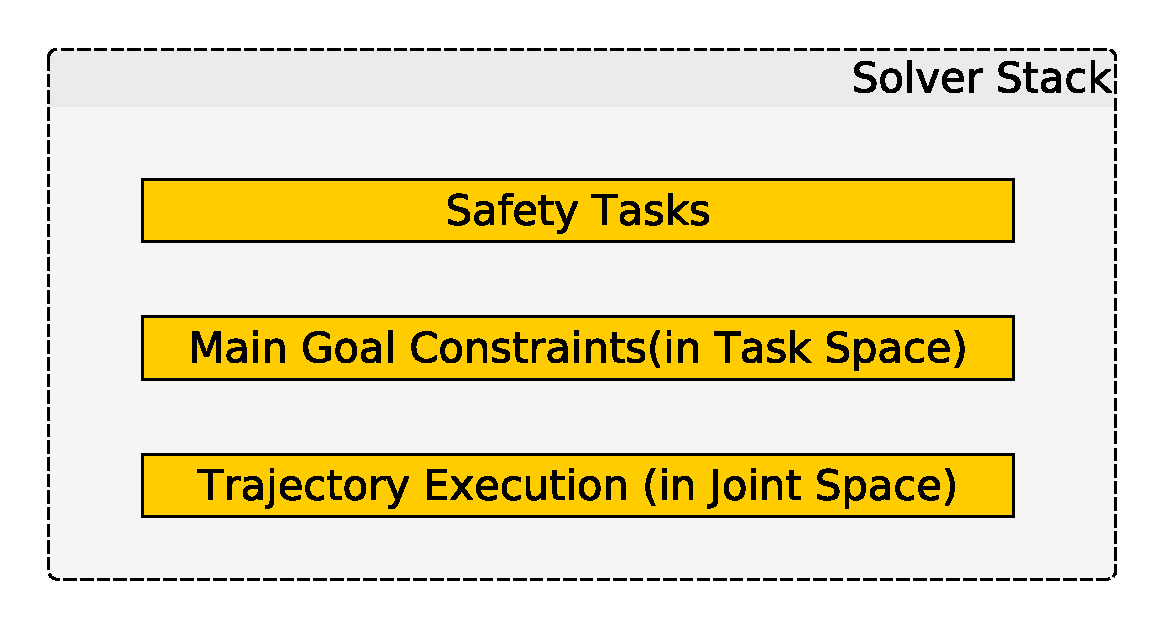
\includegraphics[scale=0.5]{chapters/doa/images/ProposedMethodology.eps}
      \caption{Generic stack order for combining planning and control. }
      \label{gso}
   \end{figure}

Safety tasks are obviously given higher priority in the stack for collision avoidance. Trajectory execution in Joint space occupies the least priority which leaves the controller only the left degrees of freedom from the primary task. If a base trajectory crosses an unforeseen or dynamic obstacle and if the sensors can sense it, the robot basically cannot execute the trajectory until the object is actually moved out of its way. Replanning could be activated if there is no other possibility to reach the joint trajectory goal. Even if there is a possibility to avoid the obstacle and continue executing the  trajectory, it is always not sure that the robot will end up in the desired goal in the task space. The clever trick here is in the way the main goals are defined. The main goal can be moving a base to a particular pose in the world or move the end effector to a grasping pose. Here the important thing is that the goals are something defined in the workspace though a joint trajectory is executed to achieve them. The hierarchical nature of the controller puts this main goal task in high priority and the jacobian core of the solver finds an optimal solution to follow the main goal. The next section illustrates this methodology on a simple scenario to show the potential of this method.


% \section{title}
Current collaborative robot solutions guarantee safety, but they use
obstacle detection to stop moving. Our dynamic obstacle avoidance
solution is that of using obstacle detection to respond by moving around the
obstacles while continuing to accomplish the desired tasks. Additionally, our integrated dynamic motion planning approach creates motion
plans that fulfil various task specific constraints for typical industrial
applications. For example the work cell 3D model is used to create a consistent
model of the work environment, so that collision free trajectories are flexibly 
generated for different operations. The automatic consideration of these
constraints  drastically simplifies and speeds-up the deployment of the robot.

An artist's illustration of our dynamic obstacle avoidance solution is shown
in Fig. \ref{fig:overview}. The robot motion control component generates
appropriate motion commands for the robot controller to follow the trajectories required for a given task. The proximity-sensing skin that covers the links and joints of the manipulator, produces information regarding potential collisions. This information is used by the robot motion control
module to adapt the robot motions on the fly to fulfil both constraints:
following the current trajectory (with a certain tolerance) and avoid
collisions. If the collision is unavoidable with local deformations of the
current trajectory, the robot motion control module requests a (global) re-planning,
which is performed on the fly by the reactive path-planner. The motion control
then takes the end effector to the final goal pose using the alternative
trajectory. The main functional modules of the system are discussed in the following
sections of the paper.

\begin{figure}[t]
\centering
\resizebox{0.8\columnwidth}{!}{\includegraphics{chapters/doa/images/overview}}
\caption[]{An artist's schematization of the FiaD Dynamic obstacle avoidance
concept is illustrated on the left side. On the right, an overview of the main
components of the solution.}
\label{fig:overview}

\end{figure}

\begin{figure}[h]
\centering
\resizebox{0.8\columnwidth}{!}{\includegraphics{figures/sensor_unit}}
\caption[]{Robot skin developed at Institute for Cognitive Systems (ICS), TUM.}
\label{fig:RobotSkin}
\vspace{-10pt}
\end{figure}	

Our robot skin system is modularized and transduces multi-modal tactile stimuli \cite{MittendorferYC15}. 
The robot skin consists of hexagonally shaped PCB modules which we call skin cells (see Fig. \ref{fig:RobotSkin}). 
A group of directly connected skin cells is termed skin patch. All skin cells are identical and contain the same set of sensors.
The sensors sample 9 tactile stimuli of 4 different
modalities, namely vibration (3D acceleration sensor), 3 normal forces (capacitive force sensor), 2 temperatures and 1 distance
(optical proximity sensor). These sensors are either off-the-shelf standard ICs or in the case of the force sensors a in-house development.
A microcontroller in the back of each skin cell collects data from its sensors, filters it and creates and sends data packets,
which contain the most recent values of all sensors. All the skin cells are connected to each other via stretchable flex PCBs 
which allows the skin to cover curved surfaces and increases its robustness. The network of skin cells is a meshed bidirectional
communication network which is routed by the microcontrollers of the skin cells. A self-organized algorithm initializes all 
the skin cells in a skin network and constructs a bidirectional communication path between each skin cell and the network root, 
the tactile section unit (TSU). The TSU converts skin network packets to standard UDP Ethernet packets and vice versa.
This allows for fast low latency connections between robot skin and PC (see Fig. \ref{fig:SkinCellNetworkArchitecture}).
\begin{figure}[t]
\centering
\resizebox{0.8\columnwidth}{!}{\includegraphics{figures/SkinCellNetwork}}\\[-15pt]
\caption[]{The skin cell network architecture and interface to the PC.}
\label{fig:SkinCellNetworkArchitecture}
\vspace{-10pt}
\end{figure}

The robot skin system also supports the auto-calibration of spatial relationships between skin cells of a skin patch covering a 3D 
surface \cite{Mittendorfer-IROS12tendorfer} such that the kinematic chain of every skin cell to the base frame can easily be determined.  

The proximity sensors used in the skin cells are infrared based sensors. The sensor emits infrared light and captures its reflections on obstacles 
in the range from 0 to 15 cm. The strength of the reflections allows the sensor to estimate the distance between the sensor and detected objects.   

\section{Combining motion Planning and control}
There are three kind of paradigms that classifies robot's architecture\cite{asada1986robot}. The first one being the deliberative architectures work on Sense-Plan-Act strategy with environment models to represent the world. They are less reliable for reactivity and human safety because an erroneous representation of world could result in an unfortunate situation. Reactive architectures work on Sense-Act strategy which encompasses the constraint based local controllers on which we had a short look. Though they are reliable for safety, they are only locally optimal and it is impossible to operate independently. The final architecture and the one we are interested is the hybrid architecture that can combine the potential advantages of both the components to successfully realize complex scenarios without compromising safety and reliability. 

The straight forward way to combine both of them is to execute a trajectory and use reactive techniques to take care of safety. If the robot hits a local minimum or a kinematic/task singularity, re-planning mode could be activated. These reactive techniques should basically deform a planned trajectory to achieve the desired goal while taking care of the safety simultaneously. The hierarchical jacobian controller in fact does trajectory deformations which is granted for free by the solver\cite{escande2014hierarchical}. The proposed method actually exploits the hierarchical nature of the solver to perform the deformations without sacrificing the main goal. 

\section{Reactive Control Framework}
The motion control is achieved using the Stack of Tasks (SoT) controller
framework \cite{Mansard2009} which employs a hierarchical jacobian control strategy eliminating the analytical inverse kinematics computation thus making it a generic controller for all robot platforms. The controller's hierarchical nature allows the robot to handle multiple kinematic tasks simultaneously exploiting the kinematic redundancy of the robot. The controller's real time capability comes from the high computational speed of the state of the art Hierarchical Quadratic Programming (HQP) solver backing it. 


A \emph{task} basically is a control law that achieves a specific objective which can be a free space task or just an inequality constraint that narrows down the workspace of the robot. The task function formalism is very well discussed in \cite{C.Samson1991}. In the context of our work, tasks generally include robot joint posture task, collision avoidance task, joint limits task and so on. The SoT framework handles the task priorities hierarchically in the real time to ensure there are no conflicts among tasks which is used to achieve dynamic obstacle avoidance without compromising on the main goal.

For example, let us consider a pick and place application in a collaborative
environment. The primary goal for this application is to enable a robot to move
to a (set of) desired pick and place locations repetitively. The pick and place
locations can be defined as posture tasks in SoT. However, a higher priority
task considering the collaborative nature of the environment is to avoid
collisions with obstacles that could be humans, for instance. Typically such a
task is modelled as an ``Inequality'' task and an eventual feasible solution (if
one exists) is computed by the solver by exploiting the kinematic redundancy of the robot. In the jargon of motion planning and control, this behaviour is similar to a \emph{local planner}.
However, it is likely that a feasible solution is not found due to the solver
converging to a local minima\footnote{This is caused by the use of task
Jacobians. For further details, please see \cite{Mansard2009}.} In such a
scenario, SoT can also be used to leverage the services of a global planner (see
Section \ref{subsec:reactive_path}) from the current robot state to the goal so
that an entirely new path is obtained which is free from collisions and
consequently allowing all the specified tasks to be achieved in the order of
their priorities. In Section \ref{sec:prelim_results}, we present the
experimental results of using the SoT controller on a practical setup and in
simulation. The SoT controller has also been configured to work with the ROS-control interface. In all these setups, the proximity information from
the artificial robot skin is used as an input to the collision avoidance task. In
the following part, we briefly present the global path planner software framework
that is used when the SoT controller hits a local minima.



\subsection{Stack of Tasks}
'Stack of Tasks' is a hierarchical jacobian-based task controller framework which implements the generalized inverse kinematic formalism by Hanafusa et Al. for local control of redundant systems\cite{hanafusa1981analysis}\cite{Mansard2009ik}. The framework in the earlier stages implemented the Siciliano's extension to handle multiple equality tasks\cite{siciliano1991general}. It has evolved to handle inequality constraints implementing the state of the art solver. The framework provides a structure that orders actives tasks to compute the control law without compromising on the task priority and control continuity. The framework provides a simple scripting interface to interact with controller components during the runtime and has a wrapper to communicate with the ROS world.


\subsection{What is a Task?}
A task basically composes a control law with a specific objective which can be such as reaching a desired joint position, avoiding obstacles in the environment, a visual servoing mechanism for grasping or so on. A task is mainly defined by the error between the desired and current feature, the error jacobian and the gain. These defined tasks are pushed into 'Stack of Tasks' which computes the control law for all the task objectives in an iterative manner\cite{mansard2007task}. 

\[\textit{e(t) = x\textsuperscript{*} - x }\]

where \textit{x} refers to the current state of a feature, \textit{x\textsuperscript{*}} refers to the reference feature.

\subsection{Redundancy Formalism}
Siciliano and Slotine proposed a systematic control framework to compute controller outputs for achieving multiple tasks in redundant systems from the redundancy formalism proposed by Hanafusa et al. The idea is, tasks are solved only in the null space of the higher priority tasks to avoid conflicts with them. This means, a task at any level has no effect on the tasks in the higher level as it uses only the left degrees of freedom. 

Let $(e_{1},J_{1})$ be a primary task  which is defined by  
\begin{equation} \label{eq:tf1}
\dot{e} = J\dot{q} 
\end{equation}
 \textit{J} referring to the Jacobian of the error velocity with respect to joint velocity at the current joint state.


\begin{equation} \label{eq:tf3}
\dot{q} = J_{1}^{+}\dot{e}_{1} + Pz
\end{equation}
 Where \textit{P} is the projector on the null space of the the Jacobian J and \textit{ $z$ } is the arbitrary velocity vector which can be used as a parameter to achieve the secondary objectives. 

Let $(e_{1},J_{1})(e_{2},J_{2})...(e_{n},J_{n})$ be tasks in the stack. The redundancy formalism for two tasks can be extended to n tasks such that $e_{i}$ does not conflict with $e_{j}$ such that $j<i$. 


The recursive joint velocity is of the form
\begin{equation} \label{eq:ntasks}
  \dot{q}_{0} = 0\\
\end{equation}
\begin{equation}
  \dot{q}_{i} = \dot{q}_{i-1}+ (J_{i}P^{A}_{i-1})^{+}(\dot{e}_{i} - J_{i}\dot{q}_{i-1}), i= 1..n
\end{equation}



 where $P^{A}_{i-1}$ is the projector onto the null space of the augmented Jacobian $J_i^A = (J_1...J_i)$ and $\widetilde{J}_i = J_iP_{i-1}^A$ is the limited jacobian of the task. The joint velocity achieving all the task objectives is $\dot{q} = \dot{q}_n$. The recursive projector is computed by 
 
 \[P^A_i = P^A_{i-1} - (J_iP_{i-1}^A)^+J^A_{i-1}  \] 
 
 This systematic way of prioritizing tasks allows simultaneous execution of multiple tasks without conflicting each other.
 
\subsection{Hierarchical Quadratic Programming}
Mansard et al. proposed an improved QP solver to manage multiple equality and inequality problems in a prioritized hierarchy to handle redundancies[15]. The solver handles equality tasks quite the same like in Siciliano's framework but the solver uses complete orthogonal decomposition(COD) instead of Sing for solving the least squares which is quite faster and efficient. The Hierarchical complete orthogonal decomposition(HCOD), a COD of the jacobian mapping for all the levels is used to compute primal optimum for all the constraints at once making it computationally faster. 

Kanoun et al. and De lasa et. al used a primal active search algorithm which is very expensive due to inefficient optimal active set search involving inappropriate activation and deactivation of constraints at each level along the cascade\cite{de2010feature}\cite{kanoun2011kinematic}. The HQP solver depends on a modified primal active search algorithm to make the optimal active set computation much more efficient. Lexicographic optimization formalism is introduced to maintain the active set at each iteration consistent with prior levels completely eliminating unnecessary constraint deactivations and activations. The solver is ten times faster than the classical solvers and can consider inequalities at any levels of the
hierarchy \cite{escande2014hierarchical}.
\subsection{Proximity Distance Gradient for Collision Avoidance}
The computation of the gradient of the proximity distance between the collision bodies inspired from \cite{escandestrictly} is required to define inequality constraints in Stack of Tasks to avoid self-collision and with external obstacles using a proximity sensor. Let $d$ be the distance between approximated collision bodies $O_1(q)$ and $O_2(q)$. The distance between these bodies and its variation is mapped to joint actuations $q$. The distance gradient can be computed by:
\[ \frac{\partial d}{\partial q} = n_d^{'}(\frac{\partial o_1(q)}{\partial q}- \frac{\partial o_2(q)}{\partial q}) \]

where $n_d^{'}$ is the unit normal distance vector while $o_1(q)$ and $o_2(q)$ are the respective closest points. The gradient of the closest point $p$ of fixed coordinates $(\rho_1(q),\rho_2(q)....\rho_l(q))$ in the local reference frame $(e_1(q),e_2(q)...,e_l(q))$ of a collision object at joint configuration $q$ is

\[\frac{\partial p}{\partial q} =  \sum_{l=1}^{d}\rho_l(q)\frac{\partial e_l(q) }{\partial q}\]

In a 3 dimensional workspace, the expression can be written as 

\[ \frac{\partial p}{\partial q} =  (x y  z)J_\omega + J_\nu \]

where $J_\omega$ is the jacobian of the rotational degrees of freedom $J_\nu$ is the jacobian of the linear degrees of freedom. In case of the external objects, the second part of the equation can be eliminated if the object is static. 

\section{KINEO}
\hypersetup{colorlinks, linkcolor=blue}
The reactive path planning software framework is based on the industry grade KineoWorks\texttrademark\footnote{See
\href{http://www.plm.automation.siemens.com/en\_us/products/open/kineo/kineoworks/index.shtml}{Kineoworks}.} path planning library from Siemens in order to provide fast and reliable robot paths. This framework has also been seamlessly integrated into the ROS-ecosystem via a ROS package called \texttt{kws\_ros\_interface} which provides the planner implementations of KineoWorks as shared objects that are readily usable in ROS-based software via the \texttt{kws\_ros\_planner} ROS node.

Robot kinematic models are provided to KineoWorks in the Unified Robot Description Format (URDF) which is a ROS standard. Furthermore, KineoWorks also accepts the standard ROS representation of a \texttt{PointCloud}\footnote{See http://wiki.ros.org/pcl} for creating collision models of dynamic obstacles in the environment. In our work, point clouds are generated in two ways. In one scenario the point clouds are generated by a standard Kinect 3D camera that is observing the immediate environment of the robot. In the other scenario, the point clouds are generated from the proximity data obtained from the Artificial Skin. Finally, the collision detection for dynamic obstacle avoidance is performed using the Kineo\texttrademark Collision Detector (KCD)\footnote{See \href{http://www.plm.automation.siemens.com/en\_us/products/open/kineo/collision-detector/index.shtml}{KCD}.}. KCD performs 3D collision detection and minimal distance analysis between triangular mesh surfaces in assembly environments. KCD has been designed specifically to minimize memory usage and take advantage of parallel processing. The complete software architecture used in our paper for the Dynamic Collision Avoidance functionality is shown in Fig. \ref{fig:arch_dca}.
\begin{figure}[t]
\centering
\includegraphics[scale=0.47]{architecture_reactive_collision_1}
% \resizebox{2\columnwidth}{!}{\includegraphics{arch_tom_3}}\\
\caption[]{Dynamic collision avoidance software architecture.}
\label{fig:dca}
\end{figure}

In the following sections we present the current results we have of using the different functionalities described.




\section{Method to combine Path Planning and Reactive Motion Control}
The methodology is based on defining the main goal as a workspace constraint and prioritizing between safety tasks and trajectory execution task (in joint space). The figure \ref{gso} gives an intuitive idea about the stack priority order .
   \begin{figure}[thpb]
      \centering
      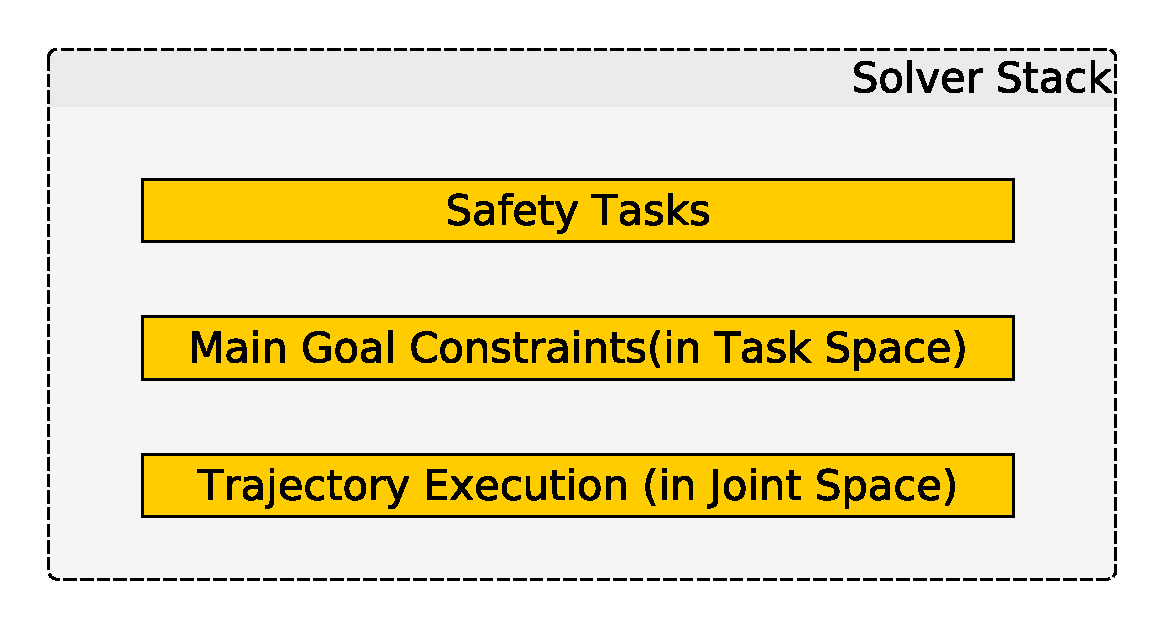
\includegraphics[scale=0.5]{chapters/doa/images/ProposedMethodology.eps}
      \caption{Generic stack order for combining planning and control. The priorities decreases from top to bottom. }
      \label{gso}
   \end{figure}

\begin{itemize}
 \item Safety tasks are obviously given higher priority in the stack for collision avoidance.
 \item Trajectory execution in Joint space occupies the least priority which leaves the controller only the left degrees of freedom from the primary task. If a base trajectory crosses an unforeseen or dynamic obstacle and if the sensors can sense it, the robot basically cannot execute the trajectory until the object is actually moved out of its way. Replanning could be activated if there is no other possibility to reach the joint trajectory goal. Even if there is a possibility to avoid the obstacle and continue executing the  trajectory, it is always not sure that the robot will end up in the desired goal in the task space. 
 
 \item The clever trick here is in the way the main goals are defined. The main goal can be moving a base to a particular pose in the world or move the end effector to a grasping pose. Here the important thing is that the goals are something defined in the workspace though a joint trajectory is executed to achieve them. The hierarchical nature of the controller puts this main goal task in high priority and the jacobian core of the solver finds an optimal solution to follow the main goal. The next section illustrates this methodology on a simple scenario to show the potential of this method.
\end{itemize}


\section{Results}
The Stack of Tasks (SoT) controller has also been deployed and tested for achieving different postures on the setup in Fig. \ref{fig:TUDSetup}. We are actively working on extending the behavior to path following and eventually integrate in accordance with the reactive collision avoidance architecture shown in Fig. \ref{fig:dca}. 


\subsection{Integrated evaluation}
\hypersetup{colorlinks, linkcolor=blue}
The integration of all the components described earlier has been evaluated on a simulation of the orange sorting setup as shown in Fig. \ref{fig:TOMMSimulation}.

\begin{figure}[h]
\centering
\resizebox{1.0\columnwidth}{!}{\includegraphics{doa/images/tomm_simulation.png}}\\[-10pt]
\caption[]{Orange sorting scenario in simulation.The red point cloud is a simulated obstacle.}
\label{fig:TOMMSimulation}
\end{figure}
The evaluation is done in a ROS based gazebo environment with the skin sensors simulated using the flexible collision library to project the distance between objects to sensor range measurements. 
These measurements are mapped to signals compatible in dynamic graph framework using a bridge component to allow its use in the SoT controller. The collision avoidance component computes the point 
distance and jacobian of each and every skin cell configured  essential to feed as an inequality constraint to the solver which backs the SoT controller. The planning component having the capability 
to plan with point cloud data has a Moveit python interface to query motion plan requests. The response is a set of way points which is then linearly interpolated to instantaneous joint position commands
to a path tracking task in the SoT. The SoT controller also has a python interface which makes it easy to design application scenarios.

The combined use of a reactive motion planner and a hierarchical reactive SoT controller with skin data makes it a good candidate for applying dynamical obstacle avoidance in factory environments.
A video result of the same is available \href{https://youtu.be/uLStjR7mpOI}{here}.

% \section{Experimental Illustration}
% We experimented a scenario to verify reactive trajectory execution to achieve a pre-grasp end effector configuration. The SOT framework is embedded in a ROS based real time controller running on a PR2, a mobile manipulation platform. The mobile base and the arms in this platform makes it apt for our scenarios which validates the practical advantage of the proposed methodology. A skin sensor is mounted on the forearm of the left arm . This scenario focuses on executing a simple trajectory on the left arm from an initial position (in the figure \ref{fig:init}) to reach a pregrasp position(in the figure \ref{fig:traj4}). The desired trajectory doesn't involve any movement in joints other than the left arm but they are not constrained to move as a part of the set-up. This figure \ref{ExperimentA} shows the tasks in the stack with priorities decreasing from top to bottom. 
%  The SOT controller executes a preplanned trajectory which is fed to the joint trajectory execution task in the stack. The respective end-effector pose of the trajectory at each instant is fed to an end effector pose task with a priority higher than the joint trajectory task.
%     \begin{figure}[h]
%       \centering
%       \includegraphics[scale=0.21]{doa/images/expillustration.png}
%       \caption{Robot Architecture of the Illustration Scenario}
%       \label{ExperimentA}
%    \end{figure}
 
% The planned way points are fed to a trajectory
% interpolator component which computes instantaneous joint position control
% signals to execute a joint posture task. The skin sensor component being a
% ROS based node publishes topics which are converted to signals in Dynamic
% Graph to be used by collision avoidance component necessary to compute
% information for feeding an inequality task in the solver stack. This is how
% safety and trajectory tracking are executed simultaneously. The adaptability of the controller without compromising the end goal comes
% from the pose task inserted between these tasks. The trajectory interpolator also sends a forward kinematic signal of the end effector corresponding to the joint trajectory point every instant. This allows the controller to stick with the
% plan as close as possible without violating the safety constraints and
% compromising the end goal of the scenario.



% \begin{figure}[!htb]
% \minipage{0.25\textwidth}
%   \includegraphics[width=\linewidth]{doa/images/traj1.png}
%   \caption{Initial Posture}\label{fig:init}
% \endminipage
% \minipage{0.25\textwidth}
%   \vspace{0.15\textwidth}
%   \includegraphics[width=\linewidth]{doa/images/traj4.png}
%   \caption{The robot while executing the trajectory with an actor's hand in proximity.}\label{fig:traj2}
% \endminipage\hfill
% \minipage{0.25\textwidth}%
%   \vspace{0.2\textwidth}
%   \includegraphics[width=\linewidth]{doa/images/traj8.png}
%   \caption{Base motion to avoid proximity with hand simulated yet the wrist pose is maintained.}\label{fig:traj3}
% \endminipage
% \minipage{0.25\textwidth}%
% \vspace{0.13\textwidth}
%   \includegraphics[width=\linewidth]{doa/images/traj11.png}
%   \caption{Final Posture after the sensor error is within the safe region.}\label{fig:traj4}
% \endminipage
% \end{figure}
   
%     \begin{figure}[!h]
%       \centering
%       \includegraphics[scale=0.35]{doa/images/BasePlot-eps-converted-to-crop.pdf}
%       \caption{Base Motion Trajectory Evolution}
%       \label{figurebase}
%    \end{figure}  
   
%   The experiment is done in simulation and the skin sensor error is varied using a software handle. The pink colored vector on the left forearm seen in the figures \ref{fig:init} -\ref{fig:traj4} correspond to unit normal distance vector determining the direction of the robot motion in the workspace to avoid collision. The figure \ref{figurebase} shows the evolution of the base position when the sensor error oscillates between safe and unsafe regions of proximity with an obstacle. They clearly shows the base motion deviating from the reference trajectory but gets back its desired state when the error is in the safe region. The important thing is the pose of the wrist is unchanged except the yaw ( which was relaxed in the pose task to afford base motion to avoid collision while it maintains the pose)
%    \begin{figure}[!h]
%       \centering
%       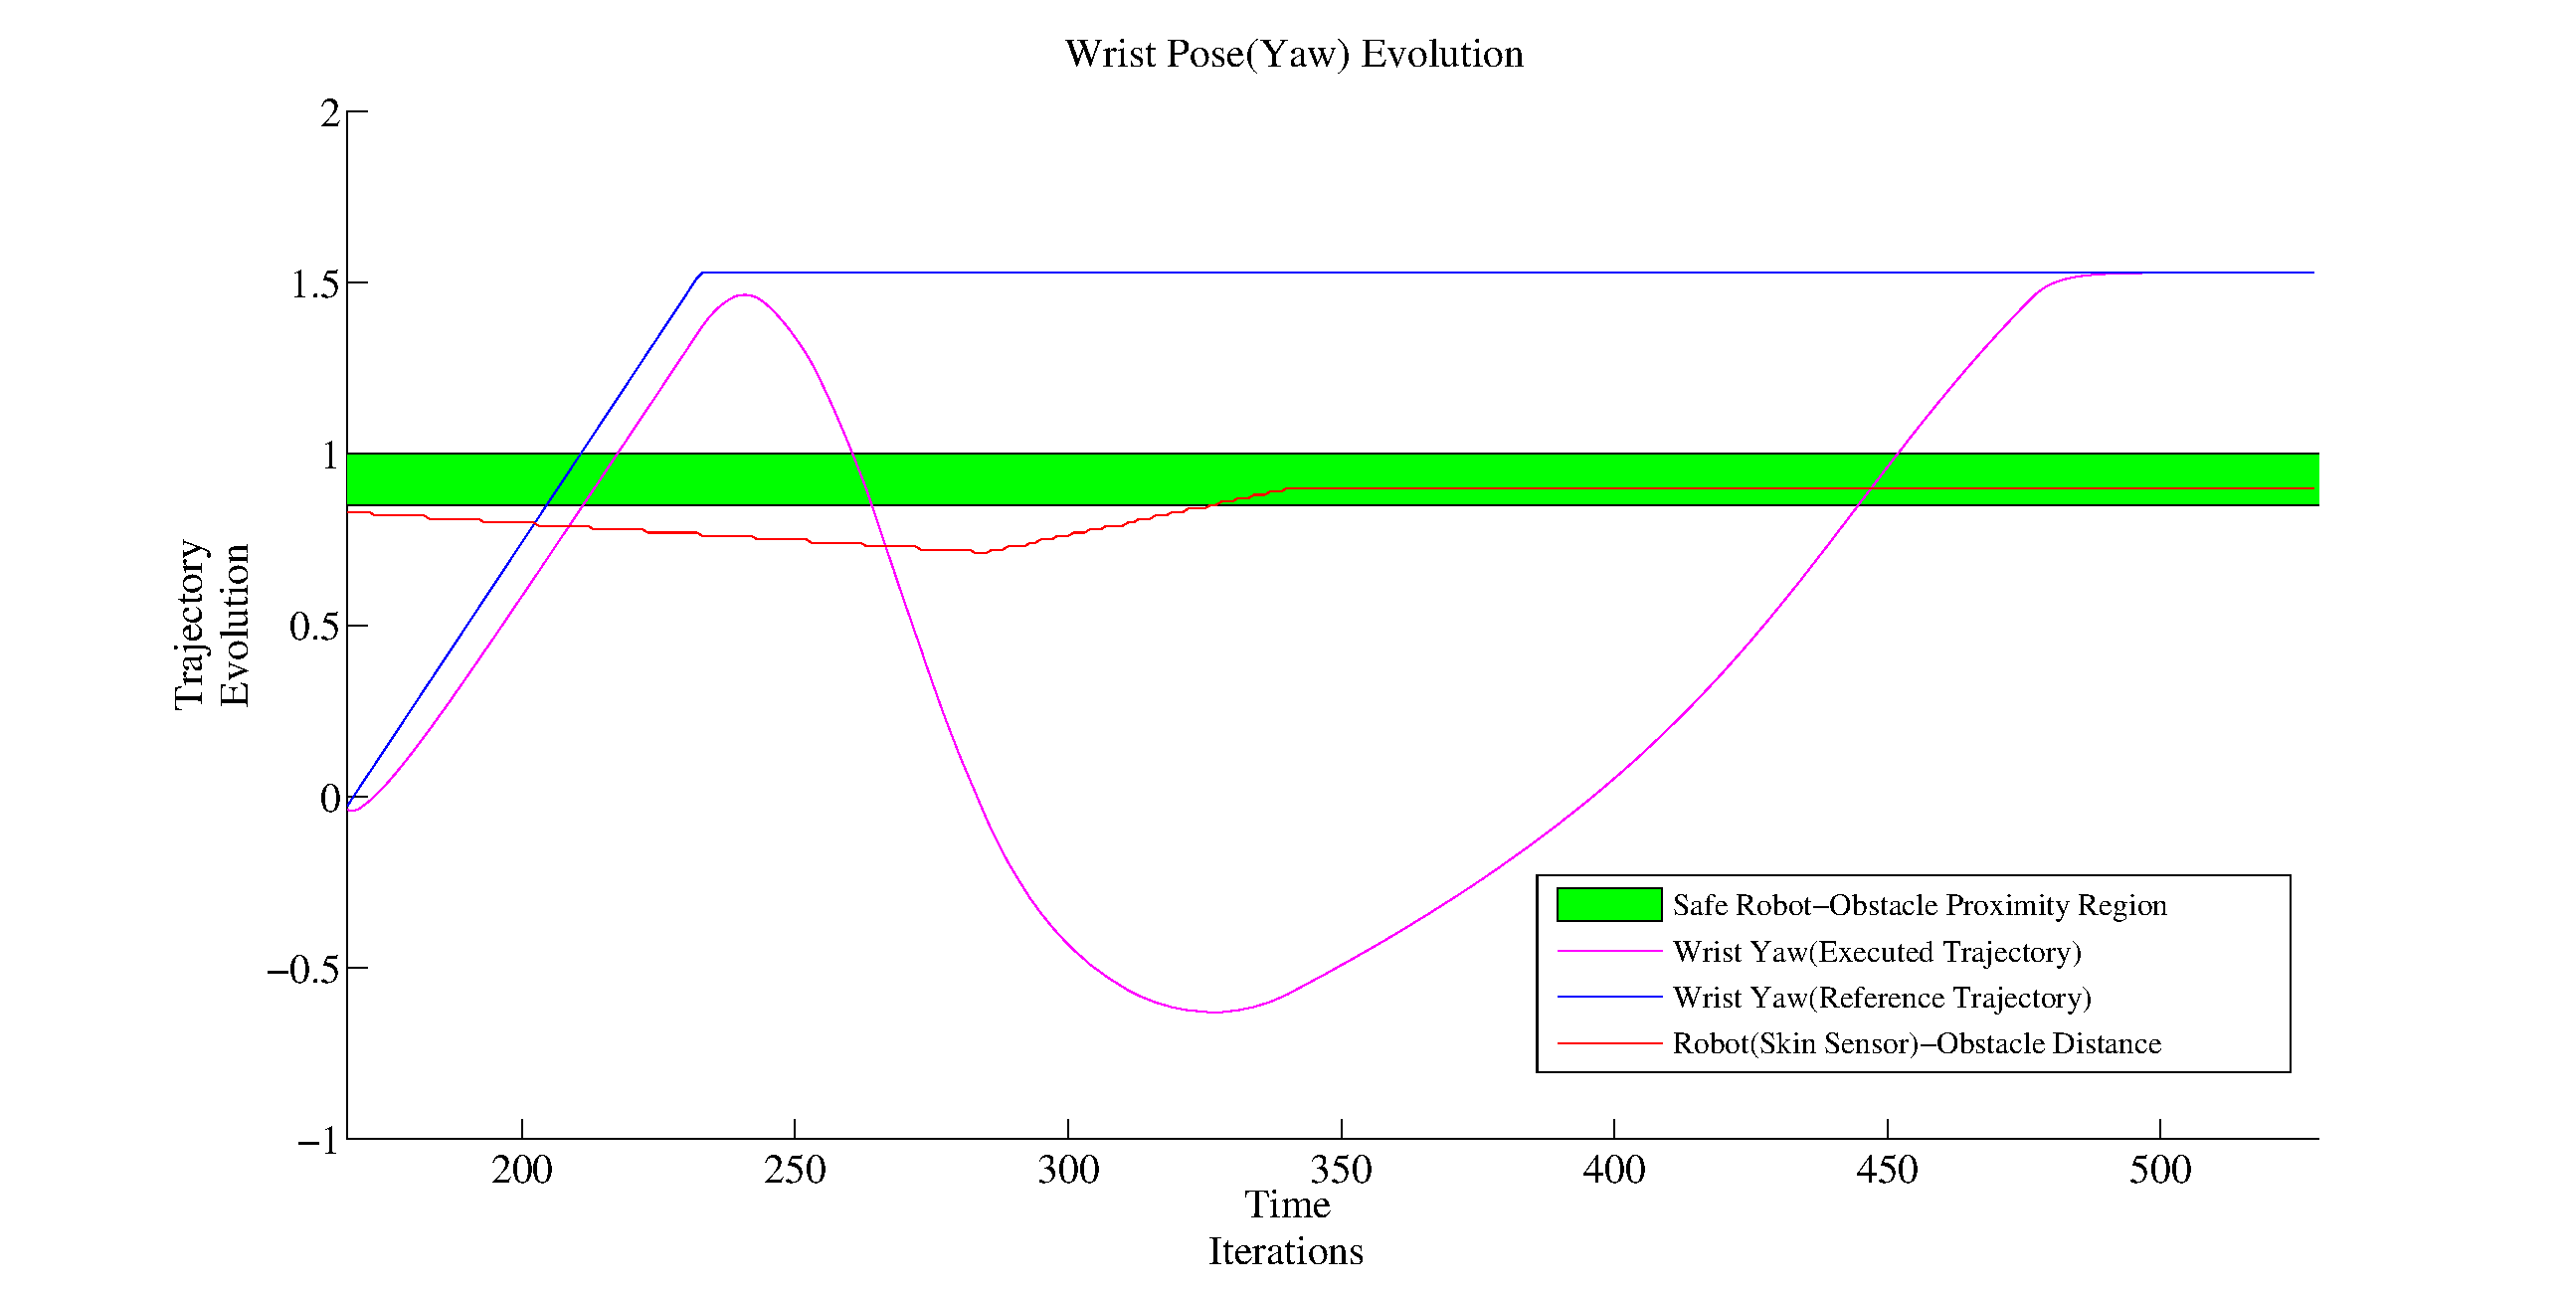
\includegraphics[scale=0.2]{doa/images/WristYawTrajectoryEvolution.eps}
%       \caption{Wrist Pose (Yaw) Evolution}
%       \label{poseYaw}
%    \end{figure}
  
% The figure \ref{poseYaw} shows the evolution of the wrist pose(yaw) of the robot which shows the connection with the base motion to compensate for the collision avoidance but yet the wrist roll and pitch in workspace doesn't change. The simple scenario could be extended to complex scenarios by figuring out the appropriate tasks corresponding to the scenario. The future work will be focused on a generic methodology to generate tasks in the stack just by specifying the scenario and feeding a trajectory.

\section{Conclusion}

This chapter presented the technologies that have been developed in the FiaD
project to augment collaborative robot manipulators with dynamic obstacle
avoidance. All these technologies: a proximity-sensing robot skin, a reactive
path planning solution and a robot motion control strategy, have been validated
in laboratory prototypes. Also, a preliminary prototype of an integrated
solution based on these technologies has been tested in simulation. With the current promising results, we are currently working on a robotic system prototype (based on the setup in Fig. \ref{fig:TUDSetup})

% work in progress%=CITE SUPPORTING EVIDENCE THAT IT WORKS=.
The integration and installation of advanced functionalities such as the dynamic
obstacle avoidance solution presented poses three main challenges from the
software point of view. The first is the integration of different components such as the skin driver, path planner and robot motion control. We address this challenge by adhering to the software development paradigm of the ROS-Industrial initiative. All the components discussed in this paper have been successfully integrated with ROS.

A second challenge is the quality assurance and robustness of the integrated robot software. This is crucial in production environments, and is specially important in collaborative applications, where safety needs to be guaranteed. For this purpose an Automated testing Framework (ATF) has been developed \cite{Weisshardt-2016} as a part of the FiaD prohect, which
allows for the systematic testing of robot software components, which includes unit
 testing, simulation-in-the-loop testing and eventually hardware-in-the-loop testing.
The tests can be automated and integrated in a centralized continuous
integration system. Preliminary test have already been conducted with the
components of the robot software system of this work, and the integrated
prototype applications will be tested with ATF.

Finally, the third challenge is the deployment of the software. One of the main barriers to transfer solutions based on robot frameworks such as ROS to industry, and specially SMEs, is how cumbersome it is
to deploy. As a part of the FiaD project, a Robot deployment toolbox has been developed \cite{Ludtke-2017}, based on ROS, which can also be integrated with ATF.
The deployment tools will also be evaluated on the RBE17 prototype.


% The paper proposed a creative method to execute a trajectory robust to run-time inequality constraints without compromising on the final goal of a scenario. The method uses 'Stack of Tasks', a jacobian control framework employing the state of the art HQP solver for both equality and inequality constraints. The creativity lies on the way the hierarchical nature of the solver and flexible task definition of the framework is exploited to combine an intuitive main goal definition and reactive trajectory execution to realize a scenario successfully robustly. Experiments were done to verify the validity of the method on a PR2 robot with a skin sensor(in simulation) mounted on its forearm. Future work will focus on generalizing the method for various kind of tasks and extending the framework to systematically design tasks to be added in the controller stack specific to possible desired scenarios. The methodology has a significant potential to be used for a robot setup with full body skin sensors.

\input{rc_inertial_params/RobustController}
\ifdefined\included
\else
\documentclass[a4paper,11pt,twoside]{StyleThese}
\usepackage{amsmath,amssymb}             % AMS Math
\usepackage[T1]{fontenc}
\usepackage[utf8x]{inputenc}
\usepackage{babel}
\usepackage{datetime}

\usepackage{lmodern}
\usepackage{tabularx}
%\usepackage{tabular}
\usepackage{multirow}

\usepackage{hhline}
\usepackage[left=1.5in,right=1.3in,top=1.1in,bottom=1.1in,includefoot,includehead,headheight=13.6pt]{geometry}
\renewcommand{\baselinestretch}{1.05}

% Table of contents for each chapter

\usepackage[nottoc, notlof, notlot]{tocbibind}
\usepackage{minitoc}
\setcounter{minitocdepth}{2}
\mtcindent=15pt
% Use \minitoc where to put a table of contents

\usepackage{aecompl}

% Glossary / list of abbreviations

\usepackage[intoc]{nomencl}
\iftoggle{ThesisInEnglish}{%
\renewcommand{\nomname}{Glossary}
}{ %
\renewcommand{\nomname}{Liste des Abréviations}
}

\makenomenclature

% My pdf code

\usepackage{ifpdf}

\ifpdf
  \usepackage[pdftex]{graphicx}
  \DeclareGraphicsExtensions{.jpg}
  \usepackage[a4paper,pagebackref,hyperindex=true]{hyperref}
  \usepackage{tikz}
  \usetikzlibrary{arrows,shapes,calc}
\else
  \usepackage{graphicx}
  \DeclareGraphicsExtensions{.ps,.eps}
  \usepackage[a4paper,dvipdfm,pagebackref,hyperindex=true]{hyperref}
\fi

\graphicspath{{.}{images/}}

%% nicer backref links. NOTE: The flag ThesisInEnglish is used to define the
% language in the back references. Read more about it in These.tex

\iftoggle{ThesisInEnglish}{%
\renewcommand*{\backref}[1]{}
\renewcommand*{\backrefalt}[4]{%
\ifcase #1 %
(Not cited.)%
\or
(Cited in page~#2.)%
\else
(Cited in pages~#2.)%
\fi}
\renewcommand*{\backrefsep}{, }
\renewcommand*{\backreftwosep}{ and~}
\renewcommand*{\backreflastsep}{ and~}
}{%
\renewcommand*{\backref}[1]{}
\renewcommand*{\backrefalt}[4]{%
\ifcase #1 %
(Non cité.)%
\or
(Cité en page~#2.)%
\else
(Cité en pages~#2.)%
\fi}
\renewcommand*{\backrefsep}{, }
\renewcommand*{\backreftwosep}{ et~}
\renewcommand*{\backreflastsep}{ et~}
}

% Links in pdf
\usepackage{color}
\definecolor{linkcol}{rgb}{0,0,0.4} 
\definecolor{citecol}{rgb}{0.5,0,0} 
\definecolor{linkcol}{rgb}{0,0,0} 
\definecolor{citecol}{rgb}{0,0,0}
% Change this to change the informations included in the pdf file

\hypersetup
{
bookmarksopen=true,
pdftitle="Évaluation de la sécurité des équipements grand public connectés à Internet",
pdfauthor="Yann BACHY", %auteur du document
pdfsubject="Thèse", %sujet du document
%pdftoolbar=false, %barre d'outils non visible
pdfmenubar=true, %barre de menu visible
pdfhighlight=/O, %effet d'un clic sur un lien hypertexte
colorlinks=true, %couleurs sur les liens hypertextes
pdfpagemode=None, %aucun mode de page
pdfpagelayout=SinglePage, %ouverture en simple page
pdffitwindow=true, %pages ouvertes entierement dans toute la fenetre
linkcolor=linkcol, %couleur des liens hypertextes internes
citecolor=citecol, %couleur des liens pour les citations
urlcolor=linkcol %couleur des liens pour les url
}

% definitions.
% -------------------

\setcounter{secnumdepth}{3}
\setcounter{tocdepth}{2}

% Some useful commands and shortcut for maths:  partial derivative and stuff

\newcommand{\pd}[2]{\frac{\partial #1}{\partial #2}}
\def\abs{\operatorname{abs}}
\def\argmax{\operatornamewithlimits{arg\,max}}
\def\argmin{\operatornamewithlimits{arg\,min}}
\def\diag{\operatorname{Diag}}
\newcommand{\eqRef}[1]{(\ref{#1})}

\usepackage{rotating}                    % Sideways of figures & tables
%\usepackage{bibunits}
%\usepackage[sectionbib]{chapterbib}          % Cross-reference package (Natural BiB)
%\usepackage{natbib}                  % Put References at the end of each chapter
                                         % Do not put 'sectionbib' option here.
                                         % Sectionbib option in 'natbib' will do.
\usepackage{fancyhdr}                    % Fancy Header and Footer

% \usepackage{txfonts}                     % Public Times New Roman text & math font
  
%%% Fancy Header %%%%%%%%%%%%%%%%%%%%%%%%%%%%%%%%%%%%%%%%%%%%%%%%%%%%%%%%%%%%%%%%%%
% Fancy Header Style Options

\pagestyle{fancy}                       % Sets fancy header and footer
\fancyfoot{}                            % Delete current footer settings

%\renewcommand{\chaptermark}[1]{         % Lower Case Chapter marker style
%  \markboth{\chaptername\ \thechapter.\ #1}}{}} %

%\renewcommand{\sectionmark}[1]{         % Lower case Section marker style
%  \markright{\thesection.\ #1}}         %

\fancyhead[LE,RO]{\bfseries\thepage}    % Page number (boldface) in left on even
% pages and right on odd pages
\fancyhead[RE]{\bfseries\nouppercase{\leftmark}}      % Chapter in the right on even pages
\fancyhead[LO]{\bfseries\nouppercase{\rightmark}}     % Section in the left on odd pages

\let\headruleORIG\headrule
\renewcommand{\headrule}{\color{black} \headruleORIG}
\renewcommand{\headrulewidth}{1.0pt}
\usepackage{colortbl}
\arrayrulecolor{black}

\fancypagestyle{plain}{
  \fancyhead{}
  \fancyfoot{}
  \renewcommand{\headrulewidth}{0pt}
}

%\usepackage{MyAlgorithm}
%\usepackage[noend]{MyAlgorithmic}
\usepackage[ED=MITT - STICRT, Ets=INSA]{tlsflyleaf}
%%% Clear Header %%%%%%%%%%%%%%%%%%%%%%%%%%%%%%%%%%%%%%%%%%%%%%%%%%%%%%%%%%%%%%%%%%
% Clear Header Style on the Last Empty Odd pages
\makeatletter

\def\cleardoublepage{\clearpage\if@twoside \ifodd\c@page\else%
  \hbox{}%
  \thispagestyle{empty}%              % Empty header styles
  \newpage%
  \if@twocolumn\hbox{}\newpage\fi\fi\fi}

\makeatother
 
%%%%%%%%%%%%%%%%%%%%%%%%%%%%%%%%%%%%%%%%%%%%%%%%%%%%%%%%%%%%%%%%%%%%%%%%%%%%%%% 
% Prints your review date and 'Draft Version' (From Josullvn, CS, CMU)
\newcommand{\reviewtimetoday}[2]{\special{!userdict begin
    /bop-hook{gsave 20 710 translate 45 rotate 0.8 setgray
      /Times-Roman findfont 12 scalefont setfont 0 0   moveto (#1) show
      0 -12 moveto (#2) show grestore}def end}}
% You can turn on or off this option.
% \reviewtimetoday{\today}{Draft Version}
%%%%%%%%%%%%%%%%%%%%%%%%%%%%%%%%%%%%%%%%%%%%%%%%%%%%%%%%%%%%%%%%%%%%%%%%%%%%%%% 

\newenvironment{maxime}[1]
{
\vspace*{0cm}
\hfill
\begin{minipage}{0.5\textwidth}%
%\rule[0.5ex]{\textwidth}{0.1mm}\\%
\hrulefill $\:$ {\bf #1}\\
%\vspace*{-0.25cm}
\it 
}%
{%

\hrulefill
\vspace*{0.5cm}%
\end{minipage}
}

\let\minitocORIG\minitoc
\renewcommand{\minitoc}{\minitocORIG \vspace{1.5em}}

\usepackage{multirow}
%\usepackage{slashbox}

\newenvironment{bulletList}%
{ \begin{list}%
	{$\bullet$}%
	{\setlength{\labelwidth}{25pt}%
	 \setlength{\leftmargin}{30pt}%
	 \setlength{\itemsep}{\parsep}}}%
{ \end{list} }

\newtheorem{definition}{Définition}
\renewcommand{\epsilon}{\varepsilon}

% centered page environment

\newenvironment{vcenterpage}
{\newpage\vspace*{\fill}\thispagestyle{empty}\renewcommand{\headrulewidth}{0pt}}
{\vspace*{\fill}}

\usepackage{tablefootnote}

\usepackage{hyperref}
\hypersetup{
     colorlinks   = true,
     citecolor    = violet
}
\usepackage{graphicx} % for pdf, bitmapped graphics files
\usepackage{amsmath} % assumes amsmath package installed
\usepackage{amssymb}  % assumes amsmath package installed
\usepackage{bm} % for using bold lowercase greek letters
\usepackage{array}
\usepackage{colortbl}	% to color table background
%\usepackage[table]{xcolor}
\usepackage{subfigure}  
\usepackage{tikz}
\newcommand{\tikzcircle}[2][red,fill=red]{\tikz[baseline=-0.5ex]\draw[#1,radius=#2] (0,0) circle ;}%
\definecolor{turquoise}{rgb}{0.28 1 0.92}
\input{rc_inertial_params/math_commands.tex}
\usepackage{epstopdf}
\usepackage[colorinlistoftodos,prependcaption,textsize=tiny]{todonotes}
\newcommand\explainmore[1]{\textcolor{red}{#1}}
\newcommand\refrephrase[1]{\textcolor{yellow}{#1}}
\newcommand\donerephrasing[1]{\textcolor{green}{#1}}

%DIF PREAMBLE EXTENSION ADDED BY LATEXDIFF
%DIF UNDERLINE PREAMBLE %DIF PREAMBLE
\RequirePackage[normalem]{ulem} %DIF PREAMBLE
\RequirePackage{color}\definecolor{RED}{rgb}{1,0,0}\definecolor{BLUE}{rgb}{0,0,1} %DIF PREAMBLE
\providecommand{\DIFadd}[1]{{\protect\color{blue}\uwave{#1}}} %DIF PREAMBLE
\providecommand{\DIFdel}[1]{{\protect\color{red}\sout{#1}}}                      %DIF PREAMBLE
%DIF SAFE PREAMBLE %DIF PREAMBLE
\providecommand{\DIFaddbegin}{} %DIF PREAMBLE
\providecommand{\DIFaddend}{} %DIF PREAMBLE
\providecommand{\DIFdelbegin}{} %DIF PREAMBLE
\providecommand{\DIFdelend}{} %DIF PREAMBLE
%DIF FLOATSAFE PREAMBLE %DIF PREAMBLE
\providecommand{\DIFaddFL}[1]{\DIFadd{#1}} %DIF PREAMBLE
\providecommand{\DIFdelFL}[1]{\DIFdel{#1}} %DIF PREAMBLE
\providecommand{\DIFaddbeginFL}{} %DIF PREAMBLE
\providecommand{\DIFaddendFL}{} %DIF PREAMBLE
\providecommand{\DIFdelbeginFL}{} %DIF PREAMBLE
\providecommand{\DIFdelendFL}{} %DIF PREAMBLE
%DIF END PREAMBLE EXTENSION ADDED BY LATEXDIFF


\begin{document}


\sloppy
\begin{document}
\fi


\chapter*{Conclusion}
\addstarredchapter{Conclusion} %Sinon cela n'apparait pas dans la table des matières

\ifdefined\included
\else
\bibliographystyle{acm}
\bibliography{These}
\end{document}
\fi
% \appendix
% \include{Annexe1}

\bibliographystyle{StyleThese}
%\bibliographystyle{plain}
\bibliography{These}

% \cleardoublepage
% \begin{vcenterpage}
% \noindent\rule[2pt]{\textwidth}{0.5pt}
% \\
% \iftoggle{ThesisInEnglish}{%
% {\large\textbf{Abstract:}}
% }{%
% {\large\textbf{Résumé :}}
% }
% resume
% \iftoggle{ThesisInEnglish}{%
% {\large\textbf{Keywords:}}
% }{%
% {\large\textbf{Mots clés :}}
% }
% mots, clefs
% \\
% \noindent\rule[2pt]{\textwidth}{0.5pt}
% \end{vcenterpage}

\end{document}
